\chapter{Vector Field}
\section{Vector field}
Consider a vector field $A^{\mu}(x)$, where the index $\mu$ is a vector index that takes on four possible values. 
Under a Lorentz transformation, we have
\[U(\Lambda)^{-1} A^{\mu}(x) U(\Lambda) = \Lambda^{\mu}_{\phantom{\mu}\nu} A^{\nu}(\Lambda^{-1}x).\]
For an infinitesimal transformation, we have
\[\delta^{\mu}_{\phantom{\mu}\nu}+\delta \omega ^{\mu}_{\phantom{\mu}\nu} = \delta^{\mu}_{\phantom{\mu}\nu} + \frac{i}{2} \delta \omega_{\rho \sigma} (\mathcal{S}_{\rm V}^{\rho \sigma})^{\mu}_{\phantom{\mu}\nu},\]
where
\[(\mathcal{S}_{\rm V}^{\rho \sigma})^{\mu}_{\phantom{\mu}\nu} \equiv -i(\eta^{\rho \mu}\delta ^{\sigma}_{\phantom{\sigma}\nu} - \eta^{\sigma \mu}\delta^{\rho}_{\phantom{\rho}\nu}).\]
It is obvious that $A^{\dagger \mu}$ is also a vector field. 
We know that $\eta^{\mu \nu}$ is invariant under Lorentz transformation, i.e.
\[\Lambda^{\mu}_{\phantom{\mu}\rho} \Lambda^{\nu}_{\phantom{\mu}\sigma} \eta^{\rho \sigma} = \eta^{\mu \nu} .\]
We can use $\eta^{\mu \nu}$ and and its inverse $\eta_{\mu\nu}$ to raise and lower vector indices of the vector field,
\[A_{\mu} \equiv \eta_{\mu \nu} A^{\nu}.\]
And we can verify the following equations:
\[\Lambda^{\mu}_{\phantom{\mu}\nu} \Lambda_{\mu}^{\phantom{\mu}\rho} = \delta^{\rho}_{\nu} .\]
\[A^{\mu}(x) = \eta^{\mu \nu} A_{\nu}(x).\]
\[\Lambda_{\mu}^{\phantom{\mu}\rho} \Lambda_{\nu}^{\phantom{\nu}\sigma} \eta_{\rho \sigma} = \eta_{\mu \nu}.\]
\[U(\Lambda)^{-1} A_{\mu}(x) U(\Lambda) = \Lambda_{\mu}^{\phantom{\mu}\nu} A_{\nu}(\Lambda^{-1}x).\]
Define $\mathcal{C}_i \equiv \frac{1}{2}\epsilon_{ijk}\mathcal{S}_{\rm V}^{jk}$, $\mathcal{D}_i \equiv \mathcal{S}_{\rm V}^{i0}$. 
For example, we have
\[(\mathcal{C}_3)_{\mu}^{\phantom{\mu}\nu} = \left(\begin{array}{rrrr}
0 & 0 & 0 & 0 \\
0 & 0 & -i & 0 \\
0 & i & 0 & 0 \\
0 & 0 & 0 & 0
\end{array}\right).\]
The eigenvectors of $\mathcal{C}_3$ are
\[\left[\left(-1, \left[\left(0,\,1,\,-i,\,0\right)\right], 1\right),
\left(1, \left[\left(0,\,1,\,i,\,0\right)\right], 1\right), \left(0,
\left[\left(1,\,0,\,0,\,0\right), \left(0,\,0,\,0,\,1\right)\right],
2\right)\right].\]
We further define $N_i \equiv \frac{1}{2}(\mathcal{C}_i-i\mathcal{D}_i)$ and $N^{\dagger}_i \equiv \frac{1}{2}(\mathcal{C}_i + i \mathcal{D}_i)$. For example, we have
\[(N_1)_{\mu}^{\phantom{\mu}\nu} = \left(\begin{array}{rrrr}
0 & -\frac{1}{2} & 0 & 0 \\
-\frac{1}{2} & 0 & 0 & 0 \\
0 & 0 & 0 & -\frac{1}{2} i \\
0 & 0 & \frac{1}{2} i & 0
\end{array}\right).\]
The eigenvectors of $N_1$ are
\[\left[\left(-\frac{1}{2}, \left[\left(1,\,1,\,0,\,0\right),
\left(0,\,0,\,1,\,-i\right)\right], 2\right), \left(\frac{1}{2},
\left[\left(1,\,-1,\,0,\,0\right), \left(0,\,0,\,1,\,i\right)\right],
2\right)\right].\]
We can conclude that vector field is in the $(2,2)$ representation of the Lie algebra of the Lorentz group.

\section{Electromagnetic field and gauge invariance}
The Lagrangian of EM field is
\[\mathcal{L} = -\frac{1}{4}F_{\mu\nu}F^{\mu\nu},\]
where
\[F_{\mu\nu} \equiv \partial_{\mu} A_{\nu} - \partial_{\nu} A_{\mu} , \quad \mbox{and} , \quad A^{\mu} \equiv (\phi,\bm{A}).\]
Explicitly,
\[F_{0i} = \dot{A}^i + \nabla_i \phi \equiv -E^i , \quad \mbox{and} , \quad F_{ij} = \nabla_i A^j - \nabla_j A^i \equiv \epsilon_{ijk}B^k.\]
We can derive the equation of motion of the EM field by variation method,
\[\partial_{\mu}F^{\mu \nu} = 0.\]
It can be rewritten in terms of $\bm{E}$ and $\bm{B}$, i.e. Maxwell equations:
\begin{eqnarray}
&\phantom{=}&\bm{\nabla} \cdot \bm{E} = 0 , \quad \frac{\partial \bm{E}}{\partial t} = \bm{\nabla} \times \bm{B} ,\nonumber \\
&\phantom{=}& \bm{\nabla} \cdot \bm{B} = 0  , \quad \frac{\partial \bm{B}}{\partial t} = - \bm{\nabla} \times \bm{E}.\nonumber
\end{eqnarray}
The massless vector field $A_{\mu}$ has 4 components, which would naively seem to tell us that the gauge field has 4 degrees of freedom.But there are two related comments which will ensure that quantizing the gauge field $A_{\mu}$ gives rise to 2 degrees of freedom, rather than 4.
\begin{itemize}
\item The field $A_0$ has no kinetic term $\dot{A_0}$ in the Lagrangian: it is not dynamical. This means that if we are given some initial data $A_i$ and $\dot{A_i}$ at a time $t_0$, then the field $A_0$ is fully determined by the equation of motion $\bm{\nabla} \cdot \bm{E} = 0$,which, expanding out,
reads
\[\nabla^2 A_0 = \bm{\nabla} \cdot \frac{\partial \bm{A}}{\partial t}.\]
Thus $A_0$ is not independent: we don't get to specify $A_0$ on the initial time slice.
\item If we transform the EM field as
\[A_{\mu} \to A_{\mu} + \partial_{\mu}\lambda(x) ,\]
we can derive that
\[F_{\mu\nu} \to F_{\mu \nu} , \quad \mathcal{L} \to \mathcal{L}.\]
The seemed infinite number of symmetries, one for each function $\lambda(x)$, is to be viewed as a redundancy in our description. That is, two states related by a gauge symmetry are to be identified: they are the same physical state. One way to see that this interpretation is necessary is to notice that Maxwell's equations are not sufficient to specify the evolution of $A_{\mu}$.The equations read,
\[(\eta_{\mu\nu} \partial^2 - \partial_{\mu} \partial_{\nu}) A^{\nu} = 0.\]
But the operator $(\eta_{\mu\nu} \partial^2 - \partial_{\mu} \partial_{\nu})$ is not invertible: it annihilates any function of
the form $\partial_{\mu} \lambda$. This means that given any initial data, we have no way to uniquely determine $A_{\mu}$ at a later time since we can't distinguish between $A_{\mu}$ and $A_{\mu} + \partial_{\mu} \lambda$. This would be problematic if we thought that $A_{\mu}$ is a physical object. However, if we're happy to identify $A_{\mu}$ and $A_{\mu} + \partial_{\mu} \lambda$ as corresponding to the same physical state, then our problems disappear. 
\end{itemize}

\noindent
The picture that emerges for the theory of electromagnetism is of an enlarged phase space, foliated by gauge orbits. All states that lie along a given gauge orbit can be reached by a gauge transformation and are identified. To make progress, we pick a representative from each gauge orbit. It doesn't matter which representative we pick after all, they're all physically equivalent. But we should make sure that we pick a ``good'' gauge, in which we cut the orbits. Here we'll look at two different gauges:
\begin{itemize}
\item Coulomb Gauge: $\bm{\nabla} \cdot \bm{A} = 0$.
\\
We can make use of the residual gauge transformations in Lorentz gauge to pick $\bm{\nabla} \cdot \dot{\bm{A}} = 0$. We
have as a consequence $A_0 = 0$. Coulomb gauge is sometimes called radiation gauge.
\item Lorentz Gauge: $\partial^{\mu} A_{\mu} = 0$.
\\
In fact this condition doesn't pick a unique representative from the gauge orbit. We're always free to make further gauge transformations with $\partial^{\mu}\partial_{\mu} \lambda = 0$, which also has non-trivial solutions. As the name suggests, the Lorentz gauge has the advantage that it is Lorentz invariant.
\end{itemize}

\section{Canonical quantization of EM field}
\subsection{Canonical quantization in Coulomb gauge}

\subsubsection{Canonical momentum and Hamiltonian}
\[\pi^0 = \frac{\partial \mathcal{L}}{\partial \dot{A_0}} = 0 , \quad  \pi^{i} = \frac{\partial \mathcal{L}}{\partial(\partial_0 A_i)} = \dot{A}^i + \nabla_i \phi = -E^i.\]
\[\mathcal{H} = \frac{1}{2}(\bm{\pi}^2 + \bm{B}^2) + (\bm{\pi} \cdot \bm{\nabla}) A_0.\]
Integration by parts can give
\[H = \int d^3x \frac{1}{2}(\bm{\pi}^2 + \bm{B}^2).\]

\subsubsection{Momentum and angular momentum}
\[P^0 = H , \quad \vec{P} = \int - \bm{\pi} \vec{\nabla} \bm{A} d^3x.\]
\[\vec{J} = - \int \bm{\pi} (\vec{x}\times \vec{\nabla} + i \vec{C})\bm{A} \; d^3x , \quad \vec{S} = -i \int \bm{\pi} \vec{C} \bm{A} \; d^3x.\]

\subsubsection{Canonical quantization}
In Coulomb gauge, we have
\[A_0 = \pi^0 = 0 , \quad \pi^i = \dot{A}^i .\]
Three pairs of $A_i$ and $\pi^i$ are not independent from each other. They must satisfy the constraint equations
\[\nabla \cdot \bm{A} = 0 , \quad \nabla \cdot \bm{\pi} = 0.\]
A reasonable quantization condition can be written as
\[[A_i(\bm{x},t),A_j(\bm{x}',t)] = 0 , \quad [\pi^i(\bm{x},t),\pi^j(\bm{x}',t)] = 0,\]
\[[A_i(\bm{x},t),\pi^j(\bm{x}',t)] = i \left( \delta^{j}_i - \frac{\partial_i \partial^j}{\nabla^2} \right) \delta(\bm{x}-\bm{x}') \equiv i \int \frac{d^3k}{(2\pi)^3} \; (\delta^j_i - \frac{k_ik^j}{\bm{k}^2})e^{i\bm{k}\cdot(\bm{x}-\bm{x}')}.\]
In this case, we can verify that
\[\dot{A}_i = -i[A_i(\bm{x},t),H] = \pi_i (\bm{x},t),\]
\[\dot{\pi}^i = -i[\pi^i(\bm{x},t),H] = \nabla^2 A^i(\bm{x},t).\]
It is consistent with the classical field equation.

\subsubsection{Fourier expansion}
\[\bm{A}(x) = \sum_{r = \pm} \int \widetilde{dp} [a_{r}(\bm{p}) \bm{\epsilon}_r(\bm{p})e^{ipx} + a^{\dagger}_{r}(\bm{p}) \bm{\epsilon}^*_r(\bm{p})e^{-ipx}].\]
We can derive from constraint condition that
\[\bm{\epsilon} \cdot \bm{p} = 0.\]
We will choose $\bm{\epsilon}$ to satisfy that
\[\bm{\epsilon}_r \cdot \bm{\epsilon}^*_s = \delta_{rs}.\]
The completeness relation for the polarization vectors is
\[\sum_{r=\pm} \epsilon_r^i(\bm{p}) \epsilon_r^{*j}(\bm{p}) = \delta^{ij} - \frac{p^ip^j}{|\bm{p}|^2}.\]
\begin{example}
If $\bm{p} = (0,0,p)$, we usually choose 
\[\bm{\epsilon}_{+} = \frac{1}{\sqrt{2}}(1,i,0) , \quad \bm{\epsilon}_{-} = \frac{1}{\sqrt{2}}(1,-i,0) .\]
$\bm{\epsilon}_{+}$ corresponds to anticlockwise rotation and it is the eigenvectors of the space-part of $\mathcal{C}_3$ with eigenvalue $+1$. $\bm{\epsilon}_{-}$ corresponds to clockwise rotation and it is eigenvector of the space-part of $\mathcal{C}_3$ with eigenvalue $- 1$.
\end{example}
\noindent
We can further derive from above discussion that
\[\bm{\pi}(x) = -i \sum_{r = \pm} \int \widetilde{dp} \omega [a_{r}(\bm{p}) \bm{\epsilon}_r(\bm{p})e^{ipx} - a^{\dagger}_{r}(\bm{p}) \bm{\epsilon}^*_r(\bm{p})e^{-ipx}];\]
\[a_r(\bm{p}) = \bm{\epsilon}^*_r \int d^3x e^{-ikx}(i\bm{\pi}+\omega\bm{A});\]
\[a^{\dagger}_r(\bm{p}) = \bm{\epsilon}_r \int d^3x e^{ikx}(-i\bm{\pi}+\omega\bm{A});\]
\[[a_r(\bm{p}),a_{r'}(\bm{p'})] = 0 , \quad [a^{\dagger}_r(\bm{p}),a^{\dagger}_{r'}(\bm{p'})] = 0 , \quad [a_r(\bm{p}),a^{\dagger}_{r'}(\bm{p'})] = (2\pi)^3 2\omega \delta_{rr'} \delta(\bm{p} - \bm{p}').\]

\subsubsection{Operator represented by $a$ and $a^{\dagger}$}
Define that
\[N(\bm{p},r) \equiv a^{\dagger}_{r}(\bm{p}) a_r(\bm{p}).\]
We can derive that
\[H = \sum_{r = \pm} \int \widetilde{dp} \; \omega N(\bm{p},r) + 2\mathcal{E}_0V,\]
\[\vec{P} = \sum_{r = \pm} \int \widetilde{dp} \; \vec{p} N(\bm{p},r) ,\]
\[\vec{S} = \sum_{r,s = \pm} \int \widetilde{dp} \; \frac{1}{2}(\bm{\epsilon}^*_{s} \vec{C}\bm{\epsilon}_{r} - \bm{\epsilon}_{r} \vec{C}\bm{\epsilon}^*_{s}) a^{\dagger}_{s}(\bm{p}) a_r(\bm{p}).\]
From above equation, we can say that $a^{\dagger}_r(\bm{p})$ create an photon with energy $\omega$, momentum $\bm{p}$ and spin angular momentum parallel($r=+$)/antiparallel($r=-$) with the direction of momentum.

\subsubsection{Propagator}
\[G_{\rm F}(x-y)_{ij} \equiv \langle 0 |T A_i(x) A_j(y) | 0 \rangle = \int \frac{d^4p}{(2\pi)^4} \frac{-i}{p^2-i\epsilon} \left(\delta_{ij} - \frac{p_ip_j}{|\bm{p}|^2}\right) e^{ip(x-y)}.\]

\subsection{Canonical quantization in Lorentz gauge}
\subsubsection{Undefined metric formalism}
Modify the Maxwell Lagrangian by introducing a new term
\[\mathcal{L} = -\frac{1}{4} F_{\mu\nu}F^{\mu\nu} - \frac{1}{2\xi} (\partial_{\mu} A^{\mu})^2.\]
The equations of motion are now
\[\partial^2 A_{\mu} - (1-\frac{1}{\xi})\partial^{\mu}(\partial \cdot A) = 0.\]
Canonical momentums are
\[\pi^0 = \frac{1}{\xi} \partial \cdot A = \frac{1}{\xi}(-\dot{A}_0 + \partial_i A^i) , \quad \pi^i = \dot{A}^i + \nabla^i A^0 = -E^i.\]
Hamiltonian is
\[\mathcal{H} = \frac{1}{2}(\bm{\pi}^2 + \bm{B}^2 - \xi \pi^0 \pi^0) + (\bm{\pi} \cdot \bm{\nabla}) A_0 + \pi^0 (\bm{\nabla} \cdot \bm{A}),\]
\[H =  \int \left[ \frac{1}{2}(\bm{\pi}^2 + \bm{B}^2 - \xi \pi^0 \pi^0) -A_0(\bm{\nabla} \cdot \bm{\pi}) + \pi^0 (\bm{\nabla} \cdot \bm{A}) \right] d^3x .\]
We remark that the above Lagrangian and the equations of motion, reduce to Maxwell theory in the gauge $\partial \cdot A = 0$. This why we say that our choice corresponds to a class of Lorenz gauges with parameter $\xi$. With this abuse of language (in fact we are not setting $\partial \cdot A = 0$, otherwise the problems would come back) the value of $\xi=1$ is known as the Feynman gauge and $\xi=0$ as the Landau gauge. From now on we will take the case of the so-called Feynman gauge, where $\xi=1$. Then the equation of motion coincide with the Maxwell theory in the Lorenz gauge. In Feynman gauge, the canonical quantization conditions can be written as
\[[A_{\mu}(\bm{x},t),A_{\nu}(\bm{x}',t)] = 0 , \quad [\pi^{\mu}(\bm{x},t),\pi^{\nu}(\bm{x}',t)] = 0 , \quad [A_{\mu}(\bm{x},t),\pi^{\nu}(\bm{x}',t)] = i\delta^{\nu}_{\mu} \delta(\bm{x}-\bm{x}').\]
We can also derive that
\[[\dot{A}_{\mu}(\bm{x},t),\dot{A}_{\nu}(\bm{x}',t)] = 0 , \quad [A_{\mu}(\bm{x},t),\dot{A}_{\nu}(\bm{x}',t)] = i\eta_{\mu\nu} \delta(\bm{x}-\bm{x}').\]

\subsubsection{Fourier expansion}
\[A(x) = \sum_{\lambda=0}^{3} \int \widetilde{dp} [a_{\lambda}(\bm{p}) \epsilon_{\lambda}(\bm{p})e^{ipx} + a^{\dagger}_{\lambda}(\bm{p}) \epsilon^*_{\lambda}(\bm{p})e^{-ipx}],\]
where $\epsilon_{\lambda \mu}$ are a set of four independent 4-vectors.  We will now make a choice for these 4-vectors. We choose $\epsilon_{1\mu}$ and $\epsilon_{2\mu}$ orthogonal to $k^{\mu}$ and $n^{\mu}$, such that
\[\epsilon_{\lambda \mu} \epsilon^{*\mu}_{\lambda'} = \delta_{\lambda \lambda'} , \quad \lambda,\lambda' = 1,2.\]
Then, we choose $\epsilon_{3\mu}$ in the plane $(k^{\mu},n^{\mu})$ and perpendicular to $n^{\mu}$ such that
\[\epsilon_{3\mu} n^{\mu} = 0 , \quad \epsilon_{3\mu} \epsilon^{*\mu}_{3} = 1.\]
Finally we choose $\epsilon_{0\mu} = n_{\mu}$. The vectors $\epsilon_{1\mu}$ and $\epsilon_{2\mu}$ are called transverse polarizations, while $\epsilon_{3\mu}$ and $\epsilon_{0\mu}$ longitudinal and scalar polarizations, respectively.
In general we can show that
\[\epsilon_{\lambda} \cdot \epsilon^*_{\lambda'} = \eta_{\lambda \lambda'} , \quad \eta^{\lambda \lambda'} \epsilon_{\lambda \mu} \epsilon^*_{\lambda' \nu} = \eta_{\mu \nu} .\]
We can further derive from above discussion that
\[\dot{A}(x) = -i \sum_{\lambda=0}^{3} \int \widetilde{dp} \omega [a_{\lambda}(\bm{p}) \epsilon_{\lambda}(\bm{p})e^{ipx} - a^{\dagger}_{\lambda}(\bm{p}) \epsilon^*_{\lambda}(\bm{p})e^{-ipx}];\]
\[ a_{\lambda}(\bm{p}) =  \eta_{\lambda \lambda'} \epsilon^*_{\lambda'} \cdot \int d^3x e^{-ipx}(i\dot{A}+\omega A);\]
\[ a^{\dagger}_{\lambda}(\bm{p}) =  \eta_{\lambda \lambda'} \epsilon_{\lambda'} \cdot \int d^3x e^{ipx}(-i\dot{A}+\omega A);\]
\[[a_{\lambda}(\bm{p}),a_{\lambda'}(\bm{p'})] = 0 , \quad [a^{\dagger}_{\lambda}(\bm{p}),a^{\dagger}_{\lambda'}(\bm{p'})] = 0 , \quad [a_{\lambda}(\bm{p}),a^{\dagger}_{\lambda'}(\bm{p'})] = (2\pi)^3 2\omega \eta_{\lambda \lambda'} \delta(\bm{p} - \bm{p}').\]

\subsubsection{Indefinite metric problem}
We introduce the vacuum state defined by
\[a_{\lambda}(\bm{p}) | 0 \rangle = 0.\]
To see the problem with the sign we construct the one-particle state with scalar polarization, that is
\[|1\rangle = \int \widetilde{dp} f(p) a^{\dagger}_{0}(\bm{p})|0\rangle \]
and work out its norm
\[\langle 1 | 1 \rangle = -\langle 0 | 0 \rangle \int \widetilde{dp} |f(p)|^2.\]
The state $| 1 \rangle$ has a negative norm.
\\ \\
To solve this problem we note that we are not working anymore with the classical Maxwell theory because we modified the Lagrangian. What we would like to do is to impose the condition $\partial \cdot A = 0$, but that is impossible as an equation for operators. We can, however, require that condition on a weaker form, as a condition only to be verified by the physical states.
More specifically, we require that the part of $\partial \cdot A$ that contains the annihilation operator (positive frequencies) annihilates the physical states,
\[\partial^{\mu} A^{+}_{\mu} | \psi \rangle = 0.\]
The states $| \psi \rangle$ can be written in the form
\[| \psi \rangle = | \psi_T \rangle | \phi \rangle,\]
where $| \psi_T \rangle$  is obtained from the vacuum with creation operators with transverse polarization and $| \phi \rangle$ with scalar and longitudinal polarization.
$\partial^{\mu} A^{+}_{\mu}$ contains only scalar and longitudinal polarizations
\[\partial^{\mu} A^{+}_{\mu} = i\sum_{\lambda=0,3} \int \widetilde{dp} a_{\lambda}(\bm{p}) (p \cdot \epsilon_{\lambda}(\bm{p}) ) e^{ipx} .\]
Therefore the previous condition becomes
\[i\sum_{\lambda=0,3} (p \cdot \epsilon_{\lambda}(\bm{p})) a_{\lambda}(\bm{p})  | \phi \rangle = 0.\]
The condition is equivalent to,
\[(a_{0}(\bm{p}) - a_{3}(\bm{p})) | \phi \rangle = 0.\]
We can construct $| \phi \rangle$ as a linear combination of states $| \phi \rangle$ with $n$ scalar or longitudinal photons:
\[| \phi \rangle = C_0 | \phi_0 \rangle + C_1 | \phi \rangle + \cdots\]
where $| \phi_0 \rangle \equiv | 0 \rangle$.
The states $|\phi_n\rangle$ are eigenstates of the operator number for scalar or longitudinal photons
\[N' | \phi_n \rangle = n | \phi_n \rangle,\]
where
\[N' \equiv \int \widetilde{dp} [a^{\dagger}_{3}(\bm{p})a_{3}(\bm{p})-a^{\dagger}_{0}(\bm{p})a_{0}(\bm{p})] .\]
Then
\[n \langle \phi_n | \phi_n \rangle = \langle \phi_n |N'| \phi_n \rangle = 0.\]
This means that
\[\langle \phi_n | \phi_n \rangle = \delta_{n0},\]
that is, for $n \neq 0$, the state $| \phi_n \rangle$ has zero norm. We have then for the general state $| \phi \rangle$,
\[\langle \phi | \phi \rangle = |C_0|^2 \geq 0\]
and the coefficients $C_i(i=1,2,\cdots)$ are arbitrary.

\subsubsection{Operator represented by $a$ and $a^{\dagger}$}
Define
\[N'(\bm{p}) \equiv a^{\dagger}_{3}(\bm{p})a_{3}(\bm{p})-a^{\dagger}_{0}(\bm{p})a_{0}(\bm{p}),\]
\[N(\bm{p},1) \equiv a^{\dagger}_{1}(\bm{p}) a_{1}(\bm{p}) , \quad N(\bm{p},2) \equiv a^{\dagger}_{2}(\bm{p}) a_{2}(\bm{p}) , \quad N_T(\bm{p}) \equiv N(\bm{p},1) + N(\bm{p},2).\]
We have
\[\langle \psi | N'(\bm{p}) | \psi\rangle = 0 , \quad \langle \psi | N_T(\bm{p}) | \psi\rangle = \langle \psi_T | N_T(\bm{p}) | \psi_T\rangle.\]
As we can derive
\[ H = \int \widetilde{dp} \; \omega [N'(\bm{p}) + N_T(\bm{p})] + 2\mathcal{E}_0V,\]
\[ \vec{P} = \int \widetilde{dp} \; \vec{p} [N'(\bm{p}) + N_T(\bm{p})],\]
the arbitrariness of $C_i(i=1,2,\cdots)$ does not affect the physical observables. Only the physical transverse polarizations
contribute to the result. Two states that differ only in their time-like and longitudinal photon content, $|\phi_n\rangle$ with $n \geq 1$ are said to be physically equivalent. We can think of the gauge symmetry of the classical theory as descending to the Hilbert space of the quantum theory.
It is important to note that although for the average values of the physical observables only the transverse polarizations contribute, the scalar and longitudinal polarizations are necessary for the consistency of the theory. In particular they show up when we consider complete sums over the intermediate states.

\subsubsection{Propagator}
\[G_{\rm F}(x-y)_{\mu\nu} \equiv \langle 0 |T A_{\mu}(x) A_{\nu}(y) | 0 \rangle = \int \frac{d^4p}{(2\pi)^4} \frac{-i\eta_{\mu\nu}}{p^2-i\epsilon}  e^{ip(x-y)}.\]
It is easy to verify that $G_{\rm F}(x-y)_{\mu\nu}$ is the Green's function of the equation of motion:
\[\partial^2 G_{\rm F}(x-y)_{\mu\nu} = i\eta_{\mu\nu}\delta(x-y).\]
For the general case, $\xi \neq 0$, the equal times commutation relations are more complicated. The propagator will be
\[G_{\rm F}(x-y)_{\mu\nu}  = \int \frac{d^4p}{(2\pi)^4} \left[\frac{-i\eta_{\mu\nu}}{p^2-i\epsilon} + i(1-\xi)\frac{p_{\mu}p_{\nu}}{(p^2-i\epsilon)^2}\right] e^{ip(x-y)}.\]

\section{Perturbation theory for canonical quantization}
\subsection{Lagrangian of QED}
\noindent
The Lagrangian of QED is
\[\mathcal{L} = -\frac{1}{4}F_{\mu\nu}F^{\mu\nu} + \overline{\Psi} (i\slashed{\partial}-m_0) \Psi + e_0j^{\mu} A_{\mu},\]
where $j^{\mu} \equiv \overline{\Psi}\gamma^{\mu}\Psi$. Usually, we also define a covariant derivative,
\[D_{\mu}\Psi \equiv \partial_{\mu}\Psi - ie_0A_{\mu}\Psi .\]
Thus the Lagrangian can also be written as
\[\mathcal{L} = -\frac{1}{4}F_{\mu\nu}F^{\mu\nu} + \overline{\Psi} (i\slashed{D}-m_0) \Psi.\]
The Lagrangian is invariant under the gauge transformation
\[A_{\mu}(x) \to A_{\mu}(x) + \frac{1}{e_0}\partial_{\mu}\alpha(x) , \quad \Psi(x) \to e^{i\alpha(x)} \Psi(x).\]

\subsection{Coulomb gauge}
The constraint equations are
\[\bm{\nabla} \cdot \bm{A} = 0 , \quad \bm{\nabla}^2 A_0 = e_0j^0.\]
The solution for $A_0$ is
\[A_0(\bm{x},t) = -e_0 \int d^3 x' \frac{j^0(\bm{x}',t)}{4\pi|\bm{x}-\bm{x}'|}.\]
Finally, we can derive that
\[H = H_{\rm D} + H_{\rm M} + H_{\mathrm{int}},\]
where,
\[H_{\rm D} \equiv \int d^3 x \; -\Pi (\vec{\alpha} \cdot \vec{\nabla} + i \beta m)\Psi , \quad H_{\rm M} \equiv \int d^3x \; \frac{1}{2}(\bm{\pi}^2 + \bm{B}^2),\]
\[H_{\mathrm{int}} \equiv \int d^3x \; \left[-e_0\bm{j}\cdot\bm{A} + \frac{e_0^2}{2} \int d^3x' \frac{j^0(\bm{x}) j^0(\bm{x}')}{4\pi|\bm{x}-\bm{x}'|} \right].\]
The perturbation expansion of correlation functions is
\[\langle \Omega | T \{\Psi(x) \overline{\Psi}(y) A(z) \} | \Omega \rangle = \lim_{T \to \infty(1-i\epsilon)} \frac{\langle 0 | T \left\{ \Psi_{\rm I}(x) \overline{\Psi}_{\rm I}(y) A_{\rm I}(z) \mathrm{exp} \left[ -i \int_{-T}^{T} dt H_{\rm I} \right]\right\} | 0 \rangle}{\langle 0 | T \left\{ \mathrm{exp} \left[ -i \int_{-T}^{T} dt H_{\rm I} \right]\right\} | 0 \rangle},\]
where $\int_{T}^{T} dt H_{\rm I}$ can be written as
\[\left[-\int d^4x e_0\overline{\Psi}_{\rm I}\bm{\gamma}\Psi_{\rm I}\cdot\bm{A}_{\rm I} \right] +\left[ \int d^4x \int d^4x' \frac{e_0^2\delta(t-t')}{4\pi|\bm{x}-\bm{x}'|}\; \frac{1}{2} \overline{\Psi}_{\rm I}(\bm{x},t)\gamma^0 \Psi_{\rm I}(\bm{x},t) \overline{\Psi}_{\rm I}(\bm{x}',t')\gamma^0 \Psi_{\rm I}(\bm{x}',t') \right].\]
Wick's theorem for photons takes is similar to that in $\phi^4$ theory:
\[T \left\{ A_{\rm I}(x_1) A_{\rm I}(x_2)  A_{\rm I}(x_3) \cdots \right\} = N \left\{A_{\rm I}(x_1) A_{\rm I}(x_2)  A_{\rm I}(x_3) \cdots + \mbox{ all possible contractions }\right\} .\]
\begin{example}
\begin{eqnarray}
&& \langle 0 | T \left\{ A_{{\rm I}i}(x_1) A_{{\rm I}j}(x_2) A_{{\rm I}k}(x_3) A_{{\rm I}l}(x_4)\right\}| 0 \rangle \nonumber \\
&=&  G_{\rm F}(x_1-x_2)_{ij} G_{\rm F}(x_3-x_4)_{kl} + G_{\rm F}(x_1-x_3)_{ik}G_{\rm F}(x_2-x_4)_{jl} +  G_{\rm F}(x_1-x_4)_{il}G_{\rm F}(x_2-x_3)_{jk} .\nonumber
\end{eqnarray}
\end{example}
\noindent
Now we can derive the Feynman rule for QED theory.
Firstly, we evaluate this term,
\[\langle 0 | T \left\{ \Psi_{{\rm I}a}(x) \overline{\Psi}_{{\rm I}b}(y) A_{{\rm I}i}(z) (i e_0) \int dw^4 \overline{\Psi}_{\rm I}(w) \bm{\gamma} \Psi_{\rm I}(w) \cdot A_{\rm I}(w) \right\} | 0 \rangle.\]
After contraction, it can be written as
\begin{eqnarray}
&-&  (ie_0) S_{\rm F}(x-y)_{ab} \int d^4 w G_{\rm F}(z-w)_{ik} \mathrm{Tr}[\gamma^k S_{\rm F}(w-w)] \nonumber \\
&+&  (ie_0) \int d^4 w G_{\rm F}(w-z)_{ik}  [S_{\rm F}(x-w) \gamma^k S_{\rm F}(w-y)]_{ab}  .\nonumber
\end{eqnarray}
It can be represented by the following Feynman diagram.
\begin{figure}[!h]
\centering
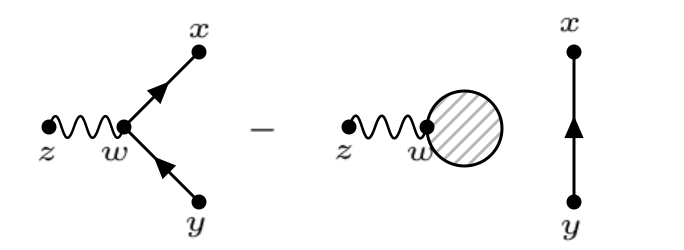
\includegraphics[scale=0.3]{QFT3/FD1.png}
\caption{Feynman diagram representation of perturbation expansion}
\end{figure}
\\
Secondly, we evaluate this term,
\[\langle 0 | T \left\{ \Psi_{{\rm I}a}(x) \overline{\Psi}_{{\rm I}b}(y) \int d^4w \int d^4w' \frac{-ie_0^2\delta(w^0-w'^0)}{4\pi|\bm{w}-\bm{w}'|}\; \frac{1}{2} \overline{\Psi}_{\rm I}(w)\gamma^0 \Psi_{\rm I}(w) \overline{\Psi}_{\rm I}(w')\gamma^0 \Psi_{\rm I}(w') \right\} | 0 \rangle.\]
After contraction, it can be written as
\begin{eqnarray}
&-&  (ie_0)^2 \int d^4w d^4w' \frac{i\delta(w^0-w'^0)}{4\pi|\bm{w}-\bm{w}'|} [S_{\rm F}(x-w)\gamma^0 S_{\rm F}(w-y)]_{ab} \mathrm{Tr}[\gamma^0 S_{\rm F}(w'-w')] \nonumber \\
&+&  (ie_0)^2 \int d^4w d^4w' \frac{i\delta(w^0-w'^0)}{4\pi|\bm{w}-\bm{w}'|} [S_{\rm F}(x-w)\gamma^0 S_{\rm F}(w-w') \gamma^0 S_{\rm F}(w'-y)]_{ab} \nonumber \\
&+& \frac{1}{2} (ie_0)^2 S_{\rm F}(x-y)_{ab} \int d^4w d^4w' \frac{i\delta(w^0-w'^0)}{4\pi|\bm{w}-\bm{w}'|} \mathrm{Tr}[\gamma^0 S_{\rm F}(w-w)] \mathrm{Tr}[\gamma^0 S_{\rm F}(w'-w')] \nonumber \\
&-& \frac{1}{2} (ie_0)^2 S_{\rm F}(x-y)_{ab} \int d^4w d^4w' \frac{i\delta(w^0-w'^0)}{4\pi|\bm{w}-\bm{w}'|} \mathrm{Tr}[\gamma^0 S_{\rm F}(w-w')\gamma^0 S_{\rm F}(w'-w)] .\nonumber
\end{eqnarray}
It can be represented by the following Feynman diagram.
\begin{figure}[!h]
\centering
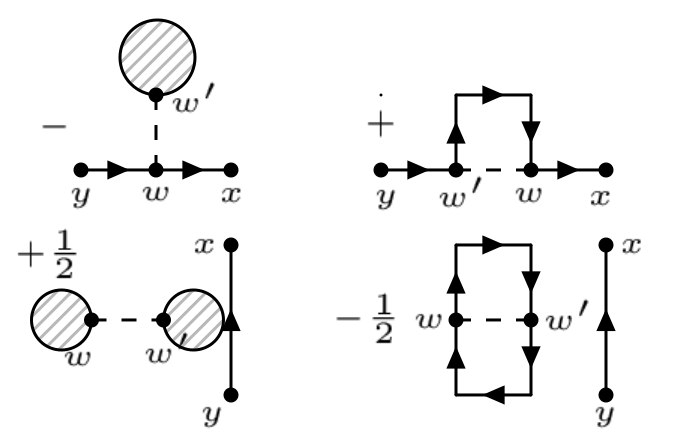
\includegraphics[scale=0.3]{QFT3/FD2.png}
\caption{Feynman diagram representation of perturbation expansion}
\end{figure}
\\
Before we write down Feynman rules, we notice that the offending non-local interaction comes from the $A_0$ component of the gauge field, we could try to redefine the propagator to include a $G_{\rm F}(x-y)_{00}$ piece which will capture this term. We can verify that
\[\frac{i\delta(w^0-w'^0)}{4\pi|\bm{w}-\bm{w}'|} = \int \frac{d^4p}{(2\pi)^4} \frac{ie^{ip(w-w')}}{|\bm{p}|^2}.\]
Thus we can combine the non-local interaction with the transverse photon propagator by defining a new photon propagator
\[G_{\rm F}(p)_{\mu\nu} \equiv \begin{cases} \frac{i}{|\bm{p}|^2} , \quad \mu,\nu=0\\  \frac{-i}{p^2-i\epsilon} \left(\delta_{ij} - \frac{p_ip_j}{|\bm{p}|^2}\right) , \quad \mu = i \neq 0, \nu = j \neq 0 \\ 0 , \quad \mbox{otherwise} \end{cases} .\]
With this propagator, the wavy photon line now carries a $\mu,\nu = 0,1,2,3$ index, with the extra $\mu=0$ component taking care of the instantaneous interaction.\\
The Feynman rules for QED are:
\begin{enumerate}
\item For each Fermion propagator from $y$ to $x$, $P = S_{\rm F}(x-y)$.
\item For each vector propagator, $P = G_{\rm F}(x-y)$.
\item For each vertex, $V = (ie_0\gamma^{\mu})\int d^4w$.
\item For each external point, $E=1$.
\item Divided by the symmetry factor.
\end{enumerate}

\subsection{Lorentz Gauge}
\noindent
In Lorentz gauge,
\[\mathcal{H}_{\rm int} = -e_0 \overline{\Psi} \gamma^{\mu} \Psi A_{\mu}.\]
The Feynman rules for QED in Lorentz gauge will be the same as that in Coulomb gauge expect for that the vector propagator will be
\[G_{\rm F}(p)_{\mu\nu}  = \frac{-i\eta_{\mu\nu}}{p^2-i\epsilon} + i(1-\xi)\frac{p_{\mu}p_{\nu}}{(p^2-i\epsilon)^2} .\]
Especially, for Feynman gauge $\xi=1$, we have
\[G_{\rm F}(p)_{\mu\nu}  = \frac{-i\eta_{\mu\nu}}{p^2-i\epsilon} .\]

\section{Path integral quantization}
\subsection{Path integral formulation for free EM field}
The correlation function is given by
\[\langle \Omega | T A_{\rm H}(x_1) A_{\rm H}(x_2)| \Omega \rangle = \lim_{T \to \infty(1-i\epsilon)} \frac{\int \mathcal{D}A \; \mathrm{exp} \left[ i\int_{-T}^T d^4x (-\frac{1}{4} F^{\mu\nu}F_{\mu\nu}) \right] A(x_1) A(x_2)}{\int \mathcal{D}A \; \mathrm{exp} \left[ i\int_{-T}^T d^4x (-\frac{1}{4} F^{\mu\nu}F_{\mu\nu}) \right]}.\]
The generating function is 
\[Z[J] = \int \mathcal{D}A \; \mathrm{exp} \left[ i\int d^4x (-\frac{1}{4} F^{\mu\nu}F_{\mu\nu}) + J^{\mu} A_{\mu} \right].\]
We can verify that
\[S = \int d^4x (-\frac{1}{4} F^{\mu\nu}F_{\mu\nu}) = \frac{1}{2} \int d^4x A_{\mu}(x) (\partial^2\eta^{\mu\nu} - \partial^{\mu}\partial^{\nu})A_{\nu}(x).\]
Notice that $(\partial^2\eta^{\mu\nu} - \partial^{\mu}\partial^{\nu})$ is singular, since for any $\alpha(x)$, 
\[(\partial^2\eta^{\mu\nu} - \partial^{\mu}\partial^{\nu})\partial_{\mu}\alpha(x) = 0.\]
This difficulty is due to gauge invariance. 
The functional is badly defined because we are redundantly integrating over a continuous infinity of physically equivalent field configurations. To fix the problem, we would like to isolate the interesting part of the functional integral, which counts each physical configuration only once.
Let $G(A)$ be some function that we wish to set equal zero as a gauge-fixing condition. We could constrain the functional integral to cover only the configurations with $G(A) = 0$ by inserting a functional delta function, $\delta(G(A))$. To do so, we insert $1$ in the path integral:
\[ 1 = \int \mathcal{D}\alpha(x) \delta(G(A(\alpha))) \det \left( \frac{\delta G}{\delta \alpha} \right),\]
where
\[A_{\mu}(\alpha(x)) = A_{\mu}(x) + \frac{1}{e_0}\partial_{\mu}\alpha(x).\]
We set the gauge fixing function as $G(A) = \partial^{\mu} A_{\mu} -\omega(x)$, so $G(A(\alpha)) = \partial^{\mu} A_{\mu} + \frac{1}{e_0}\partial^2 \alpha - \omega(x)$. It is obvious that $\det \left( \frac{\delta G}{\delta \alpha} \right)$ is equivalent to $\det(\partial^2)/e_0$, which is independent of $A$. Thus
\[Z[0] = \det \left( \frac{\delta G}{\delta \alpha} \right) \int \mathcal{D}\alpha \int \mathcal{D}A e^{iS[A]} \delta(G(A(\alpha))).\]
Now change variables from $A$ to $A(\alpha)$. This is a simple shift, so $\mathcal{D}A = \mathcal{D}A(\alpha)$. Also, by gauge invariance, $S[A] = S[A(\alpha)]$. Since $A(\alpha)$ is now just a dummy integration variable, we can rename it bake to $A$. Then we have
\[Z[0] = \det \left( \frac{\delta G}{\delta \alpha} \right) \int \mathcal{D}\alpha \int \mathcal{D}A e^{iS[A]} \delta(\partial^{\mu}A_{\mu} - \omega(x)).\]
Since the above equation is hold for any $\omega(x)$, we have
\begin{eqnarray}
Z[0] &=& N(\xi) \int \mathcal{D}\omega \exp\left[ -i \int d^4x \frac{\omega^2}{2\xi} \right] \frac{\det(\partial^2)}{e_0} \int \mathcal{D}\alpha \int \mathcal{D}A e^{iS[A]} \delta(\partial^{\mu}A_{\mu} - \omega(x)) \nonumber \\
&=& N(\xi) \frac{\det(\partial^2)}{e_0} \int \mathcal{D}\alpha \int \mathcal{D}A e^{iS[A]} \exp\left[ -i \int d^4x \frac{1}{2\xi} (\partial^{\mu}A_{\mu})^2\right] \nonumber \\
&=& W(\xi) \int \mathcal{D}A \exp\left[ \frac{i}{2} \int d^4x  A_{\mu} (\partial^2\eta^{\mu\nu} - \partial^{\mu}\partial^{\nu} + \frac{1}{\xi} \partial^{\mu} \partial^{\nu})A_{\nu}\right] .\nonumber
\end{eqnarray}
We rewrite the generating function as
\[Z[J] = W(\xi) \int \mathcal{D}A \exp\left[ \frac{i}{2} \int d^4x  A_{\mu} (\partial^2\eta^{\mu\nu} - \partial^{\mu}\partial^{\nu} + \frac{1}{\xi} \partial^{\mu} \partial^{\nu})A_{\nu} + J^{\mu} A_{\mu}\right].\]
Define
\[A'(x) \equiv A(x) - i \int d^4y G_{\rm F}(x-y)J(y).\]
Recall that
\[(\partial^2\eta^{\mu\nu} - \partial^{\mu}\partial^{\nu} + \frac{1}{\xi} \partial^{\mu} \partial^{\nu})G_{\rm F}(x-y)_{\nu \rho} = i\delta^{\mu}_{\rho}\delta(x-y).\]
We can derive that
\[Z[J]=Z[0] \exp \left[ -\frac{1}{2} \int d^4x d^4y J^{\mu}(x) G_{\rm F}(x-y)_{\mu\nu}J^{\nu}(y) \right].\]
The two point correlation functions are
\[\langle 0 | T A_{\rm H}(x_1) A_{\rm H}(x_2)| 0 \rangle = Z[0]^{-1} \left(-i \frac{\delta}{\delta J(x_1)} \right) \left(-i \frac{\delta}{\delta J(x_2)} \right) Z[J]\bigg|_{J=0} = G_{\rm F}(x_1-x_2) .\]

\subsection{Perturbation theory for path integral quantization}
\noindent
We use QED theory as an example:
\[\mathcal{L} = -\frac{1}{4}F_{\mu\nu}F^{\mu\nu} + \overline{\Psi} (i\slashed{\partial}-m_0) \Psi + e_0\overline{\Psi}\gamma^{\mu}\Psi A_{\mu}.\]
The Lagrangian of QED is invariant under a general gauge transformation. 
And we also notice that the measure $\mathcal{D}\Psi \mathcal{D}\overline{\Psi}$ is invariant under gauge transformation.
By the similar method, we can show that
\[Z[0] \equiv \int \mathcal{D}A \mathcal{D}\Psi \mathcal{D}\overline{\Psi}e^{iS[A,\Psi,\overline{\Psi}]} = W(\xi)\int \mathcal{D}A \mathcal{D}\Psi \mathcal{D}\overline{\Psi}e^{iS[A,\Psi,\overline{\Psi}]} \exp\left[ -i \int d^4x \frac{1}{2\xi} (\partial^{\mu}A_{\mu})^2\right] .\]
Define
\[\mathcal{L}_0 \equiv -\frac{1}{4}F_{\mu\nu}F^{\mu\nu} - \frac{1}{2\xi} (\partial^{\mu}A_{\mu})^2 + \overline{\Psi} (i\slashed{\partial}-m_0) \Psi , \quad \mathcal{L}_1 \equiv e_0\overline{\Psi}\gamma^{\mu}\Psi A_{\mu}.\]
We have
\begin{eqnarray}
Z[J] &=& W(\xi) \int \mathcal{D}A \mathcal{D}\overline{\Psi} \mathcal{D}\Psi e^{i\int d^4x [\mathcal{L}_0 + \mathcal{L}_1 + JA + \overline{\eta}\Psi + \overline{\Psi}\eta]} \nonumber \\
&=& W(\xi) e^{i\int d^4x \mathcal{L}_1(\frac{1}{i} \frac{\delta}{\delta J(x)},\frac{1}{i}\frac{\delta}{\delta \overline{\eta}(x)},-\frac{1}{i}\frac{\delta}{\delta \eta(x)})} \int \mathcal{D}\phi \mathcal{D}\overline{\Psi} \mathcal{D}A e^{i\int d^4y [\mathcal{L}_0 + JA + \overline{\eta}\Psi + \overline{\Psi}\eta]} \nonumber \\
&\propto & e^{i\int d^4x \mathcal{L}_1(\frac{1}{i} \frac{\delta}{\delta J(x)},\frac{1}{i}\frac{\delta}{\delta \overline{\eta}(x)},-\frac{1}{i}\frac{\delta}{\delta \eta(x)})} \mathrm{exp} [- \int d^4y d^4z  \frac{1}{2} J(y)G_{\rm F}(y-z)J(z) + \overline{\eta}(y)S_{\rm F}(y-z)\eta(z)] \nonumber \\
& =& \sum_{V=0}^{\infty} \frac{1}{V!} [ie_0 \int d^4x (\frac{1}{i} \frac{\delta}{\delta J^{\mu}(x)} \cdot -\frac{1}{i}\frac{\delta}{\delta \eta(x)} \cdot \gamma^{\mu} \cdot  \frac{1}{i}\frac{\delta}{\delta \overline{\eta}(x)})]^V \nonumber \\
&\times & \sum_{P_1=0}^{\infty} \frac{1}{P_1!} [-\frac{1}{2} \int d^4y_1 d^4z_1 J(y_1)G_{\rm F}(y_1-z_1)J(z_1)]^{P_1} \nonumber \\
&\times &  \sum_{P_2=0}^{\infty} \frac{1}{P_2!} [-\int d^4y_2 d^4z_2 \overline{\eta}(y_2)S_{\rm F}(y_2-z_2)\eta(z_2)]^{P_2} .\nonumber
\end{eqnarray}
If we focus on a term with particular values of $V$, $P_1$ and $P_2$, then the number of surviving scalar sources is $E_1 = 2P_1-V$, the number of surviving fermion sources is $E_2 = 2P_2-2V$.
We can introduce Feynman diagrams as in the $\phi^4$ theory. In these diagrams, a wavy line segment stands for a vector propagator $G_{\rm F}(x-y)$, a line with an arrow pointing from $y$ to $x$ for a fermion propagator $S_{\rm F}(x-y)$, a filled circle at one end of a wavy line segment for a vector source $i\int d^4x J(x)$, a filled circle at the start of a line with an arrow for a fermion source $i\int d^4x \eta(x)$, a filled circle at the end of a line with an arrow for a anti-fermion source $i\int d^4x \overline{\eta}(x)$, a vertex joining three line segments for $ie_0\gamma^{\mu}\int d^4x$.

\subsection{Ward-Takahashi identity (1)}
The Noether current of the symmetry $\Psi \to e^{i\alpha}\Psi$ is $j^{\mu} = \overline{\Psi}\gamma^{\mu}\Psi$. Recall the conservation law in functional formalism
\[\langle \partial_{\mu} j^{\mu}(x) \phi(x_1)\cdots\phi(x_n) \rangle  = \sum_{i=1}^{n} \langle \phi(x_1) \cdots (i\Delta \phi(x_i)\delta(x-x_i)) \cdots \phi(x_n) \rangle.\]
We can write the charge conservation law as
\[ie_0\partial_{\mu} \langle \Omega | T j^{\mu} \Psi(x_1) \overline{\Psi}(x_2)| \Omega\rangle = -ie_0\delta(x-x_1)\langle \Omega | T \Psi(x_1) \overline{\Psi}(x_2)| \Omega\rangle + ie_0\delta(x-x_2)\langle \Omega | T \Psi(x_1) \overline{\Psi}(x_2)| \Omega\rangle.\]
Notice that $ie_0\langle \Omega | T j^{\mu} \Psi(x_1) \overline{\Psi}(x_2)| \Omega\rangle$ can be represented by following Feynman diagram.
\begin{figure}[!h]
\centering
\includegraphics[scale=0.2, trim = 10 150 10 150]{QFT3/WI1.eps}
\caption{Feynman diagram representation of correlation function}
\end{figure}
\\
From the diagram, we have
\[\langle A_{\nu}(y) \rangle = \int d^4x G_{\rm F}(x-y)_{\mu\nu} ie_0\langle j^{\mu}(x) \rangle  = \int \frac{d^4p}{(2\pi)^4} e^{-ipy} G_{\rm F}(p)_{\mu\nu} \int d^4x e^{ipx} ie_0\langle j^{\mu}(x) \rangle.\]
Thus
\[\int d^4y \langle A_{\nu}(y) \rangle e^{iky} = G_{\rm F}(k)_{\mu\nu} \int d^4x e^{ikx} ie_0\langle j^{\mu}(x)\rangle.\]
Compute the Fourier transformation of the equation of charge conservation by integrating
\[\int d^4x e^{ikx} \int d^4x_1 e^{-iqx_1} \int d^4x_2 e^{ipx_2}.\]
We can get the so called Ward-Takahashi identity, represented by following Feynman diagram.
\begin{figure}[!h]
\centering
\includegraphics[scale=0.4, trim = 10 250 10 250]{QFT3/WI2.eps}
\caption{Feynman diagram representation of Ward identity}
\end{figure}
\\
Note that in the diagram above, the external leg of photon will be cut-off, but external leg of fermion will remain.
The above equation can be generated to the diagram with $n$ external fermions. 
%\begin{figure}[!h]
%\centering
%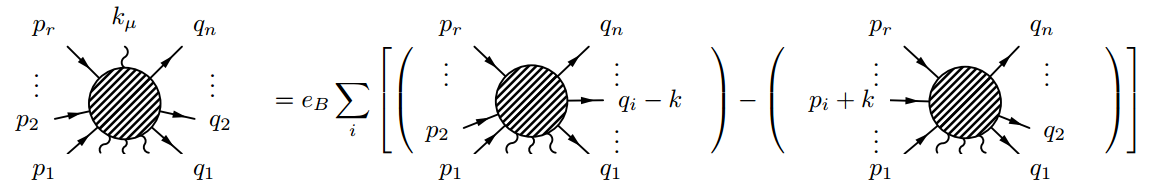
\includegraphics[height=1.87cm ,width=11.63cm]{QFT3/WI3.png}
%\caption{Feynman diagram representation of Ward identity}
%\end{figure}\
Another proof of Ward-Takahashi identity by analysing Feynman diagrams directly can be found in chapter 7.4 of \emph{An introduction to quantum field theory (M.E.Peskin \& D.V.Schroeder)}

\section{Exact propagator of photon}
\subsection{Photon self-energy}
\noindent
The exact propagator of photon is
\[\mathcal{G}(x)_{\mu\nu} = \langle  \Omega | T A_{\mu}(x)A_{\nu}(0)| \Omega \rangle_C.\]
\begin{figure}[!htb]
\centering
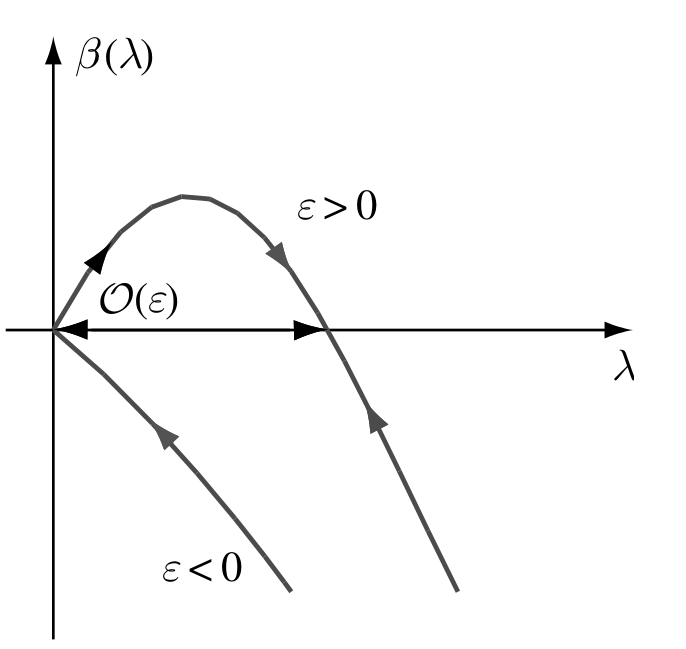
\includegraphics[scale=0.3]{QFT3/RG1.png}
\caption{Feynman diagram representation of exact propagator of photon}
\end{figure}
\\
Let us define $i\Pi^{\mu\nu}$ to be the sum of all 1-particle-irreducible insertions into the photon propagator.
We have
\[\mathcal{G}(k) = G_{\rm F}(k) + G_{\rm F}(k)(i\Pi(k))G_{\rm F}(k) + \cdots = G_{\rm F}(k) \frac{1}{1-i\Pi(k)G_{\rm F}(k)}.\]
Hence,
\[(i\mathcal{G})^{-1} = (iG_{\rm F})^{-1} - \Pi.\]
Recall that
\[iG_{\rm F}(p)_{\mu\nu}  = \frac{\eta_{\mu\nu}}{k^2-i\epsilon} - (1-\xi)\frac{k_{\mu}k_{\nu}}{(k^2-i\epsilon)^2} = \frac{1}{k^2-i\epsilon}(P^T_{\mu\nu} + \xi P^L_{\mu\nu}),\]
where 
\[P^T_{\mu\nu} \equiv \eta_{\mu\nu} - \frac{k_{\mu}k_{\nu}}{k^2} , \quad  P^L_{\mu\nu} \equiv \frac{k_{\mu}k_{\nu}}{k^2}.\]
We can derive that
\[(iG_{\rm F})^{-1}_{\mu\nu} = k^2 (P^T_{\mu\nu} + \frac{1}{\xi} P^L_{\mu\nu}).\]
We may also decompose $i\Pi^{\mu\nu}$ as
\[\Pi^{\mu\nu} = P_T^{\mu\nu}f_T(k^2) +  P_L^{\mu\nu}f_L(k^2) = \eta^{\mu\nu}f_T + \frac{k^{\mu}k^{\nu}}{k^2}(f_L-f_T).\]
Therefore,
\[(i\mathcal{G})^{-1}_{\mu\nu} = (k^2-f_T(k^2))P^T_{\mu\nu} + (\frac{k^2}{\xi}-f_L(k^2)) P^L_{\mu\nu},\]
\[\mathcal{G}(k)_{\mu\nu} = \frac{-i}{k^2-f_T(k^2)}P^T_{\mu\nu} + \frac{-i}{\frac{k^2}{\xi}-f_L(k^2)} P^L_{\mu\nu}.\]
We observe that if $f_{T,L}(k^2 = 0) \neq 0$, a mass will be generated for the photon. Because $\Pi(k)$ comes from 1PI diagrams, it should not be singular at $k^2 =0 $, and so $f_L - f_T = O(k^2)$, as $k \to 0$. We will show that gauge invariance ensures that no mass is generated from the loop corrections.

\subsection{Ward identities(2)}
We define the generating functional for connected diagrams by
\[Z[J,\eta,\overline{\eta}] = e^{-iE[J,\eta,\overline{\eta}]}.\]
Thus
\[\mathcal{G}(x-y)_{\mu\nu} = i  \frac{\delta^2 E[J,\eta,\overline{\eta}]}{\delta J^{\mu}(x) \delta J^{\nu}(y)}\bigg|_{J,\eta,\overline{\eta}=0}.\]
For infinitesimal gauge transformations, we have $\delta A_{\mu} = \partial_{\mu} \lambda $, $\delta \Psi = ie_0\lambda\Psi$ and $\delta \overline{\Psi}  = -ie_0 \lambda \overline{\Psi}$. 
Under a change of variables in the path integral, $Z[J,\eta,\overline{\eta}]$ will remain the same. 
Recall that
\[Z[J,\eta,\overline{\eta}] = W(\xi) \int \mathcal{D}A \mathcal{D}\overline{\Psi} \mathcal{D}\Psi e^{i\int d^4x [\mathcal{L}_0 + \mathcal{L}_1 + JA + \overline{\eta}\Psi + \overline{\Psi}\eta]} .\]
The change of action is
\[\delta S = -\frac{1}{\xi} \int d^4x \partial_{\mu} A^{\mu} \partial^2 \lambda + \int d^4x J^{\mu}\partial_{\mu}\lambda + ie_0\overline{\eta}\Psi\lambda - ie_0\overline{\Psi}\eta\lambda.\]
Hence, we must have
\[\int d^4x \lambda(x) W(\xi)\int \mathcal{D}A \mathcal{D}\overline{\Psi} \mathcal{D}\Psi e^{iS} \left[ -\frac{1}{\xi} \partial^2 \partial_{\mu} A^{\mu} - \partial_{\mu}J^{\mu}  + ie_0(\overline{\eta}\Psi - \overline{\Psi}\eta)\right] = 0 .\]
Since
\[\langle A_{\mu}(x) \rangle_{J,\eta,\overline{\eta}} = - \frac{\delta E}{\delta J^{\mu}} , \quad \langle \Psi(x) \rangle_{J,\eta,\overline{\eta}} = - \frac{\delta E}{\delta \overline{\eta}} , \quad \langle \overline{\Psi}(x) \rangle_{J,\eta,\overline{\eta}} =  \frac{\delta E}{\delta \eta},\]
the above equation can be written as
\[\frac{1}{\xi} \partial^2 \partial^{\mu}\frac{\delta E}{\delta J^{\mu}} - \partial_{\mu}J^{\mu} - ie_0\left[ \overline{\eta}\frac{\delta E}{\delta \overline{\eta}} + \frac{\delta E}{\delta \eta} \eta \right]=0.\]
By differentiation, we can get
\[\frac{1}{\xi} \partial^2 \partial^{\mu} \frac{\delta^2 E[J,\eta,\overline{\eta}]}{\delta J^{\mu}(x) \delta J^{\nu}(y)}\bigg|_{J,\eta,\overline{\eta}=0} - \partial_{\nu} \delta(x-y) = 0,\]
that is,
\[\frac{i}{\xi}\partial^2 \partial^{\mu} \mathcal{G}(x-y)_{\mu\nu}+ \partial_{\nu} \delta(x-y) = 0 ,\]
or, written in momentum-space,
\[-\frac{i}{\xi}k^2 k^{\mu} \mathcal{G}(k)_{\mu\nu}+ k_{\nu} = 0.\]
Thus
\[- \frac{k^2}{k^2-\xi f_L(k^2)} k_{\nu} + k_{\nu} = 0,\]
which means $f_L(k^2) =0$ and we have $f_T(k^2) \to O(k^2)$ as $k^2 \to 0$. 
The exact propagator of photon is
\[\mathcal{G}(k)_{\mu\nu} = \frac{-i}{k^2(1-\pi(k^2))}P^T_{\mu\nu} + \frac{-i\xi}{k^2} P^L_{\mu\nu},\]
where $\pi(k^2) \equiv {f_T(k^2)}/{k^2}$.

\section{LSZ reduction formula}
\subsection{LSZ reduction formula and Feynman rules}
\noindent
Suppose that the probability for the quantum field to create or annihilate an exact one-particle eigenstate of $H$ is $Z_3$, i.e.
\[\langle \Omega | A(0) | p,\lambda \rangle = \sqrt{Z_3} \epsilon_{\lambda}(p).\]
In Feynman gauge, because the norm of $|p,0\rangle$ is negative, the expansion of orthogonal complete set will be written as
\[\frac{d^3q}{(2\pi)^3} \frac{1}{2E_q} \eta^{\lambda\lambda'} | p,\lambda\rangle\langle p, \lambda' |.\]
We have demonstrated that photon will remain massless when interacting with charged fermions. Recall that $\sum_{\lambda}\xi_{\lambda}(p)\xi^{*}_{\lambda}(p) = \eta_{\mu\nu}$. 
We can derive by the similar method in $\phi^4$ theory that
\[\int d^4x \; e^{-ipx} \langle \Omega | T A_{\mu}(x) A_{\nu}(0) | \Omega \rangle_C = \frac{-iZ_3\eta_{\mu\nu}}{p^2-i\epsilon} + \cdots \]
The LSZ reduction formula for photons would take the form as follows.

\begin{newthem}[LSZ reduction formula]
\begin{eqnarray}
&\phantom{=}& \langle \bm{p}_1 \cdots \bm{p}_n \; | S | \; \bm{k}_1 \cdots \bm{k}_m \; \rangle  
\nonumber \\
&=& \prod_1^n \int d^4 x_i e^{-i p_ix_i } \prod_1^m \int d^4 y_j e^{ik_jy_j} 
\nonumber \\
&\times & \left( \frac{i}{\sqrt{Z}_3} \right) ^{m+n}  [p_1^2 \epsilon^{*\mu_1}_{\lambda_1}(p_1)] \cdots [p_n^2 \epsilon^{*\mu_n}_{\lambda_n}(p_n)] [k_1^2 \epsilon^{ \nu_1}_{\lambda'_1}(k_1)] \cdots [k_m^2 \epsilon^{ \nu_m}_{\lambda'_m}(p_m)]
\nonumber \\
&\times & \langle \Omega | T \{A_{\mu_1}(x_1) \cdots A_{\mu_n}(x_n)
A_{\nu_1}(y_1) \cdots A_{\nu_m}(y_m) \} | \Omega \rangle.
\nonumber
\end{eqnarray}
\end{newthem}

\noindent
The LSZ reduction formula in other gauge would give similar procedure for calculating scattering amplitude: Fourier transform the Green function in position space to momentum space, cut-off the external legs and multiply the polarization vector of asymptotic states. (Note there is still an extra factor $\sqrt{Z_3}^{m+n}$ to multiply, similar to the $\phi^4$ theory).
Finally, we list the Feynman rules of QED in momentum space as follows:
\begin{enumerate}
\item For each incoming electron, draw a solid line with an arrow pointed towards the vertex, and label it with the electron's four-momentum, $p_i$.
\item For each outgoing electron, draw a solid line with an arrow pointed away from the vertex, and label it with the electron's four-momentum, $p'_i$.
\item For each incoming positron, draw a solid line with an arrow pointed away from the vertex, and label it with minus the positron's four-momentum, $-p_i$.
\item For each outgoing positron, draw a solid line with an arrow pointed towards the vertex, and label it with minus the positron's four-momentum, $-p'_i$.
\item For each incoming photon, draw a wavy line with an arrow pointed towards the vertex, and label it with the photon's four-momentum,$k_i$.
\item For each outgoing photon, draw a wavy line with an arrow pointed away from the vertex, and label it with the photon's four-momentum, $k'_i$.
\item The only allowed vertex joins two solid lines, one with an arrow pointing towards it and one with an arrow pointing away from it, and one wavy line. Using this vertex, join up all the external lines, including extra internal lines as needed. In this way, draw all possible diagrams that are topologically inequivalent.
\item Assign each internal line its own four-momentum. Think of the four-momenta as flowing along the arrows, and conserve four-momentum at each vertex. 
\item The value of a diagram consists of the following factors:
\begin{itemize}
\item for each incoming photon, $\epsilon^{\mu}_{\lambda}(k)$; 
for each outgoing photon, $\epsilon^{*\mu}_{\lambda}(k)$;
\item for each incoming electron, $u_{r}(k)$; for each outgoing electron, $\overline{u}_{s}(p)$;
\item for each incoming positron, $\overline{v}_{\overline{r}}(\overline{k})$; for each outgoing positron, $v_{\overline{s}}(\overline{p})$;
\item for each vertex, $ie_0 \gamma^{\mu}$;
for each internal photon, $G_{\rm F}(p)$;
for each internal fermion, $S_{\rm F}(p)$.
\end{itemize}
\item Spinor indices are contracted by starting at one end of a fermion line: specifically, the end that has the arrow pointing away from the vertex. The factor associated with the external line is either $\bar{u}$ or $\bar{v}$. Go along the complete fermion line, following the arrows backwards, and write down (in order from left to right) the factors associated with the vertices and propagators that you encounter. The last factor is either a $u$ or $v$. Repeat this procedure for the other fermion lines, if any. The vector index on each vertex is contracted with the vector index on either the photon propagator (if the attached photon line is internal) or the photon polarization vector (if the attached photon line is external).
\item The overall sign of a tree diagram is determined by drawing all contributing diagrams in a standard form: all fermion lines horizontal, with their arrows pointing from left to right, and with the left endpoints labeled in the same fixed order (from top to bottom); if the ordering of the labels on the right endpoints of the fermion lines in a given diagram is an even (odd) permutation of an arbitrarily chosen fixed ordering, then the sign of that diagram is positive (negative).
\item Each closed fermion loop contributes an extra minus sign.
\item Value of $i\mathcal{M}$ is given by a sum over the values of the contributing diagrams.
\item $\langle f | S | i \rangle = (Z_2)^{\frac{n_f}{2}} (Z_3)^{\frac{n_p}{2}} i\mathcal{M}\delta(\sum p_f -\sum p_i)$.
\end{enumerate}

\subsection{Ward Takahashi identity (3)}
Suppose the invariant matrix element for a process is $\mathcal{M}$, if we replace the polarization state vector $\epsilon_{\lambda}^{\mu}$ (or $\epsilon_{\lambda}^{*\mu}$) of one incoming (or outgoing) photon with its momentum vector $k^{\mu}$, we have
\[k^{\mu} \mathcal{M}_{\mu} = 0.\]
\begin{newproof}
Without losing generality, we can consider a physical process with a single incoming and outgoing fermion lines respectively. Therefore, the ward identities states that
\[-ik_{\mu} F^{\mu}(k;p,q) = ie_0\left[F_0(p+k,q)-F_0(p,q-k)\right].\]
Here, $F$ keeps the external fermion legs but cuts external photon lines. According to the LSZ reduction formula, from each diagram we can get the contribution to an S matrix element by taking the coefficient of the product of poles
\[\left( \frac{-i}{\slashed{p}+m} \right) \left( \frac{-i}{\slashed{q}+m} \right).\] 
But the terms on the right hand side contain one of these poles, but neither contains both poles. Thus they contribute nothing to S-matrix. 
Thus we can have
\[k^{\mu} \mathcal{M}_{\mu} = 0.\] 
\end{newproof}

\noindent
We also note that when calculating invariant matrix element, the main difference between different gauge are photon propagator. In Coulomb gauge, we have
\[G_{\rm F}(p)_{\mu\nu} \equiv \begin{cases} \frac{i}{|\bm{p}|^2} , \quad \mu,\nu=0\\  \frac{-i}{p^2-i\epsilon} \left(\delta_{ij} - \frac{p_ip_j}{|\bm{p}|^2}\right) , \quad \mu = i \neq 0, \nu = j \neq 0 \\ 0 , \quad \mbox{otherwise} \end{cases} .\]
In Lorentz gauge, we have
\[G_{\rm F}(p)_{\mu\nu}  = \frac{-i\eta_{\mu\nu}}{p^2-i\epsilon} + i(1-\xi)\frac{p_{\mu}p_{\nu}}{(p^2-i\epsilon)^2} .\]
We now argue that they lead to the same $\mathcal{M}$ element.
For a general process, it can be represented as follows.

\begin{figure}[!h]
\centering
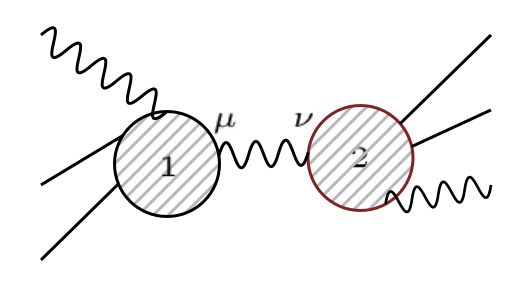
\includegraphics[scale=0.3]{QFT3/WI4.png}
\caption{Feynman diagram representation of a QED process}
\end{figure}

\noindent
The value of the diagram is
\[\mathcal{M}_{1}^{\mu} G_{\rm F}(k)_{\mu\nu}\mathcal{M}_{2}^{\nu}\]
and $k_{\mu}\mathcal{M}_{1}^{\mu}=0$, $k_{\nu}\mathcal{M}_{2}^{\nu}=0$.
The factor $\xi$ in Lorentz gauge is irrelevant to the value of $\mathcal{M}$. 
As for Coulomb gauge, denote $\mathcal{M}_{1}^{\mu}$ as $\alpha^{\mu}$, $\mathcal{M}_{2}^{\mu}$ as $\beta^{\mu}$, so 
\[\alpha^{\mu} G_{\rm F}(k)_{\mu\nu} \beta^{\nu} = i\left( -\frac{\bm{\alpha} \cdot \bm{\beta}}{k^2} + \frac{(\bm{\alpha}\cdot\bm{k})(\bm{\beta}\cdot\bm{k})}{k^2 \bm{k}^2} + \frac{\alpha^0 \beta^0 }{\bm{k}^2} \right).\]
Using the fact that $\bm{\alpha}\cdot\bm{k} + \alpha^0 k_0 = 0$, we can verify that
\[\alpha^{\mu} G_{\rm F}(k)_{\mu\nu} \beta^{\nu} = \alpha^{\mu} \left( -\frac{i\eta_{\mu\nu}}{k^2} \right)\beta^{\nu}.\]
Thus the invariant matrix element is gauge invariant.

\section{Renormalization}
\subsection{Renormalized quantum electrodynamics}
The Lagrangian of QED is
\[\mathcal{L} = -\frac{1}{4}F_{\mu\nu}F^{\mu\nu} + \overline{\Psi} (i\slashed{\partial}-m_0) \Psi + e_0j^{\mu} A_{\mu}.\]
Suppose the number of external photons is $N_{\gamma}$, the number of external fermions is $N_{e}$, the number of vertex is $V$. The superficial divergence is
\[D = 4 -N_{\gamma} - \frac{3}{2}N_{e}.\]
Recall that charge conjugation $C$ is a symmetry of QED, so $C|\Omega\rangle = | \Omega \rangle$. 
But $j^{\mu}$ changes sign under charge conjugation, $C j^{\mu}(x)C^{\dagger} = - j^{\mu}(x)$, so its vacuum expectation value must vanish:
\[\langle \Omega | T j^{\mu}(x) | \Omega \rangle = \langle \Omega | T C^{\dagger}C j^{\mu}(x)C^{\dagger}C | \Omega \rangle = -\langle \Omega | T j^{\mu}(x) | \Omega \rangle = 0 .\]
The amplitude with $N_{\gamma} = 1,N_{e}=0$ will vanish as well. 
Similarly, we can verify that the diagram with $N_{\gamma} = 3,N_e=0$ will also vanish.
As for the amplitude with $N_{\gamma} = 4$, the superficial divergence $D = 0$. Thus the only divergence must be of the form $\log \Lambda$. But the ward identity implies that
\[k^{\mu}\mathcal{M}_{\mu\nu\sigma\rho} = 0.\]
Thus the divergent terms must vanish.
If we neglect the vacuum term with $N_{\gamma}=0,N_{e}=0$, there are only three divergent amplitude terms left. We need four counter terms to eliminate all the divergence.
\begin{figure}[!h]
\centering
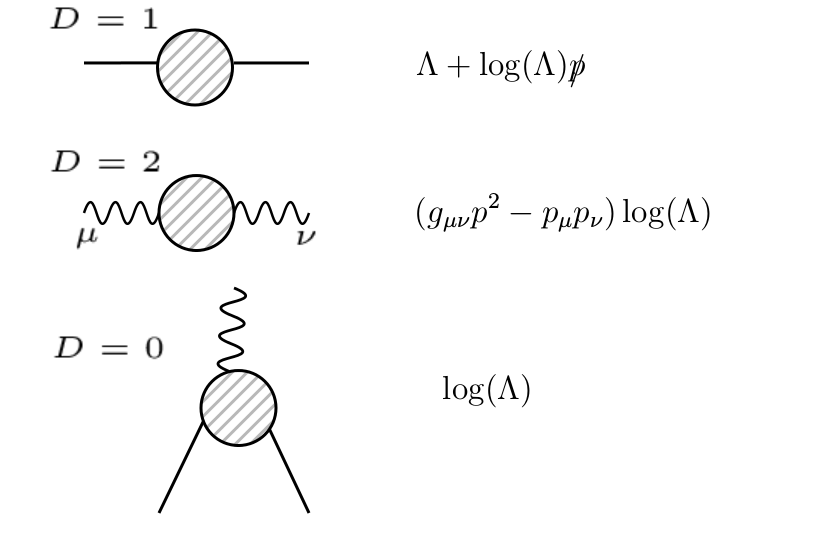
\includegraphics[scale=0.3]{QFT3/RG2.png}
\caption{Feynman diagram representation of divergent amplitude in QED}
\end{figure}
The Lagrangian can be written as
\[\mathcal{L} = \mathcal{L}_1 + \mathcal{L}_{ct},\]
where
\[\mathcal{L}_1 = -\frac{1}{4}F_r^{\mu\nu}F_{r\mu\nu} +  i\overline{\Psi}_r \gamma^{\mu} \partial_{\mu} \Psi_r - m \overline{\Psi}_r \Psi_r + e \overline{\Psi}_r\gamma^{\mu}\Psi_r A_{r\mu} ,\]
\[\mathcal{L}_{ct} = -\frac{1}{4}\delta_3 F_r^{\mu\nu}F_{r\mu\nu} + i\delta_{2}\overline{\Psi}_r \gamma^{\mu} \partial_{\mu} \Psi_r - \delta_m \overline{\Psi}_r \Psi_r + e \delta_1 \overline{\Psi}_r\gamma^{\mu}\Psi_r A_{r\mu} ,\]
\[A = \sqrt{Z_3}A_r , \quad \Phi  = \sqrt{Z_2}\Phi_r , \quad \delta_{3} = Z_3 - 1 , \quad \delta_{2} = Z_2 - 1 , \quad \]
\[\delta_m = Z_2 m_0 - m  , \quad \delta_1 = Z_1 - 1 =(e_0/e) Z_2 Z_3^{\frac{1}{2}} - 1.\]
The Feynman rules of counter terms are:
\[-\frac{1}{4}\delta_3 F_r^{\mu\nu}F_{r\mu\nu} , \quad  -i(\eta^{\mu\nu}q^2-q^{\mu}q^{\nu})\delta_3,\]
\[i\overline{\Psi}_r (\delta_{2}\slashed{\partial} - \delta_m)\Psi_r , \quad -i(\delta_2\slashed{p}+\delta_m).\]
\[ e \delta_1 \overline{\Psi}_r\gamma^{\mu}\Psi_r A_{r\mu} , \quad  \quad ie \gamma^{\mu}\delta_1 . \quad  \quad   \quad \]
We also denote the renormalized 1PI component of exact propagator of photon as $i(\eta^{\mu\nu}q^2 -q^{\mu}q^{\nu})\Pi_r(q^2)$, the renormalized 1PI component of exact propagator of fermion as $-i\Sigma_r(\slashed{p})$, the renormalized exact amputated photon-fermion-antifermion vertex as $ie\Gamma^{\mu}_r(p,p')$. 
\\ \\
Renormalized exact propagator of photon is
\[\mathcal{G}_r(q)_{\mu\nu} = \frac{-i}{q^2(1-\Pi_r(q^2))}P^T_{\mu\nu}.\]
Renormalized exact propagator of fermion is
\[\mathcal{S}_r(p) = \frac{-i}{\slashed{p}+m+\Sigma_r(\slashed{p})}.\]
The on-shell renormalization conditions are
\begin{eqnarray}
\Sigma_r(\slashed{p}=-m\gamma^0) &=& 0 ,\nonumber \\
\frac{d}{d\slashed{p}} \Sigma_r(\slashed{p}) \Big|_{\slashed{p} = -m\gamma^0} &=& 0 ,\nonumber \\
\Pi_r(q^2 = 0) &=& 0 ,\nonumber \\
ie\Gamma^{\mu}_r(p=p',p^2=-m^2) &=& ie\gamma^{\mu} ,\nonumber
\end{eqnarray}
Recall the ward identity, we have
\begin{eqnarray}
&\phantom{=}& ieZ_2\partial_{\mu} \langle \Omega | T j_r^{\mu} \Psi_r(x_1) \overline{\Psi}_r(x_2)| \Omega\rangle \nonumber \\
&=& -ie\delta(x-x_1)\langle \Omega | T \Psi_r(x_1) \overline{\Psi}_r(x_2)| \Omega\rangle + ie\delta(x-x_2)\langle \Omega | T \Psi_r(x_1) \overline{\Psi}_r(x_2)| \Omega\rangle .\nonumber
\end{eqnarray}
In momentum space, we have
\[-k_{\mu} Z_2 Z_1^{-1} \mathcal{S}_r(p+k) [ie\Gamma^{\mu}_r(p+k,p)] \mathcal{S}_r(p) \frac{1}{1-\Pi_r(k^2)} = e(\mathcal{S}_r(p+k) - \mathcal{S}_r(p)) .\]
Thus
\[Z_2 Z_1^{-1} k_{\mu} [\Gamma^{\mu}_r(p+k,p)] \frac{1}{1-\Pi_r(k^2)} =\slashed{k}+\Sigma_r(\slashed{k}+\slashed{p})-\Sigma_r(\slashed
{p}).\]
Since $\Gamma_r$, $\Pi_r$ and $\Sigma_r$ are all finite by renormalization, $Z_1/Z_2$ must be finite.
In $\overline{\rm MS}$ renormalization scheme, we immediately get
\[Z_1 = Z_2.\]
In on-shell renormalization scheme, taking the limit of $k \to 0$ and $p^2 = -m^2$, we can also get that
\[Z_1 = Z_2.\]
Therefore we have
\[e = \sqrt{Z_3}e_0.\]
This means that the relation between the bare and renormalized electric charge depends only on the photon field strength renormalization, not on quantities particular to the fermions, leading to a universal electric charge which has the same value for all species.
In the following subsection, we would omit the subscript $r$ unless it is necessary to emphasis the difference of bare field and renormalized fields.

\subsection{One loop structure of QED}
\subsubsection{Photon propagator}
\begin{figure}[!h]
\centering
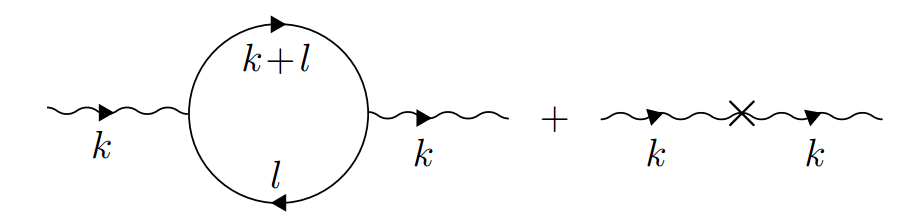
\includegraphics[scale=0.3]{QFT3/RG3.png}
\caption{The one-loop and counterterm corrections to the photon propagator}
\end{figure}
\[\Pi(k^2) = -\frac{e^2}{\pi^2} \int_0^1 dx x(1-x) \left[ \frac{1}{\epsilon} - \frac{1}{2}\ln(\frac{D}{\mu^2})\right] - \delta_3 + O(e^4),\]
where $D = x(1-x)k^2+m^2-i\epsilon$ and $\mu^2 = 4\pi e^{-\gamma} \tilde{\mu}^2$.
Impose the OS renormalization condition $\Pi(0) = 0$, we have
\[\delta_3 = -\frac{e^2}{6\pi^2} \left[ \frac{1}{\epsilon} - \ln(\frac{m}{\mu})\right] + O(e^4),\]
\[\Pi(k^2) = \frac{e^2}{2\pi^2} \int_0^1 dx x(1-x) \ln(\frac{D}{m^2}) + O(e^4).\]

\subsubsection{Fermion propagator}
The exact renormalized fermion propagator in OS renormalization can be written in Lehmann–Kallen form as
\[i\mathcal{S}(\slashed{p}) = \frac{1}{\slashed{p}+m-i\epsilon} + \int_{m_{th}}^{\infty} ds \frac{\rho_{\Psi}(s)}{\slashed{p}+\sqrt{s}-i\epsilon}.\]
We see that the first term has a pole at $\slashed{p}=-m$ with residue one. This residue corresponds to the field normalization that is needed for the validity of the LSZ formula.
There is a problem, however: in quantum electrodynamics, the threshold mass $m_{th}$ is $m$, corresponding to the contribution of a fermion and a zero energy photon. Thus the second term has a branch point at $\slashed{p}=-m$. The pole in the first term is therefore not isolated, and its residue is ill defined.
\\ \\
This is a reflection of an underlying infrared divergence, associated with the massless photon. To deal with it, we must impose an infrared cutoff that moves the branch point away from the pole. The most direct method is to change the denominator of the photon propagator from $k^2$ to $k^2+m_{\gamma}^2$, where $m_{\gamma}$ is a fictitious photon mass. Ultimately, we must deal with this issue by computing cross sections that take into account detector inefficiencies. 
In quantum electrodynamics, we must specify the lowest photon energy $\omega_{min}$ that can be detected. Only after computing cross sections with extra undetectable photons, and then summing over them, is it safe to take the limit $m_{\gamma} \to 0$. 
\begin{figure}[!h]
\centering
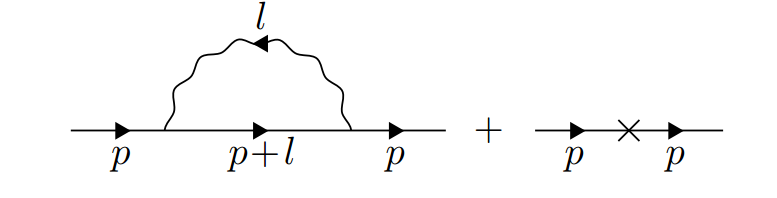
\includegraphics[scale=0.3]{QFT3/RG4.png}
\caption{The one-loop and counterterm corrections to the fermion propagator}
\end{figure}
\[\Sigma(\slashed{p}) = \frac{e^2}{8\pi^2} \int_0^1 dx \left( (2-\epsilon)(1-x)\slashed{p} + (4-\epsilon)m \right) \left[ \frac{1}{\epsilon} - \frac{1}{2}\ln(\frac{D}{\mu^2})\right] + \delta_2 \slashed{p} + \delta_m + O(e^4) ,\]
where $D = x(1-x)p^2 + xm^2 + (1-x)m_{\gamma}^2$.
The fitness of $\Sigma(\slashed{p})$ requires that
\[\delta_2 =  - \frac{e^2}{8\pi^2} \left( \frac{1}{\epsilon} + \mbox{ finite } \right) + O(e^4),\]
\[\delta_m/m = - \frac{e^2}{2\pi^2} \left( \frac{1}{\epsilon} + \mbox{ finite } \right) + O(e^4) .\]
Impose the OS renormalization condition $\Sigma(-m) = 0$ and $\Sigma'(-m) = 0$, we have
\[\Sigma(\slashed{p}) = -\frac{e^2}{8\pi^2} \int_0^1 dx \left( (1-x)\slashed{p} + 2m \right) \ln(\frac{D}{D_0})  + \kappa_2( \slashed{p} + m) + O(e^4) ,\]
where $D_0 = x^2m^2 +(1-x)m_{\gamma}^2$ and $\kappa_2 = -2 \ln(m/m_{\gamma})+1$. 

\subsubsection{Vertex}
\begin{figure}[!h]
\centering
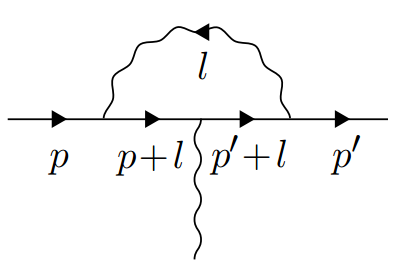
\includegraphics[scale=0.3]{QFT3/RG5.png}
\caption{The one-loop correction to the photon-fermion-fermion vertex}
\end{figure}
\[\Gamma^{\mu}(p,p') = (1+\delta_1)\gamma^{\mu} + \frac{e^2}{8\pi^2} \left[\left(\frac{1}{\epsilon} - 1 - \frac{1}{2} \int dF_3 \ln (D/\mu^2)\right)\gamma^{\mu} + \frac{1}{4} \int dF_3 \frac{\tilde{N}^{\mu}}{D}\right] + O(e^4),\]
where
\[\int dF_3 = 2 \int_0^1 dx_1 dx_2 dx_3 \delta(x_1+x_2+x_3-1),\]
\[D = x_1(1-x_1)p^2 + x_2(1-x_2)p'^2 - 2x_1x_2p \cdot p' + (x_1+x_2)m^2 + x_3 m_{\gamma}^2,\]
\[\tilde{N}^{\mu} = \gamma_{\nu}[x_1\slashed{p}-(1-x_2)\slashed{p}'+m]\gamma^{\mu}[-(1-x_1)\slashed{p}+x_2\slashed{p}'+m]\gamma^{\nu}.\]
Fitness of $\Gamma^{\mu}$ requires that
\[\delta_1 = -  \frac{e^2}{8\pi^2}(\frac{1}{\epsilon}+\mbox{ finite }) + O(e^4).\]
Impose the OS renormalization condition $\Gamma^{\mu}_r(p=p',p^2=-m^2) = \gamma^{\mu}$, we have
\[\Gamma^{\mu}(p,p') = \gamma^{\mu} - \frac{e^2}{16\pi^2} \int dF_3 \left[\left(\ln (D/D_0)+2\kappa_1\right)\gamma^{\mu} - \frac{\tilde{N}^{\mu}}{2D}\right] + O(e^4),\]
where
\[D_0 = (1-x_3)^2m^2 + x_3 m_{\gamma}^2 , \quad \kappa_1 = -2 \ln(m/m_{\gamma}) + \frac{5}{2}.\]

\subsubsection{Vertex function}
Consider the process of electron-electron scattering.
\begin{figure}[!h]
\centering
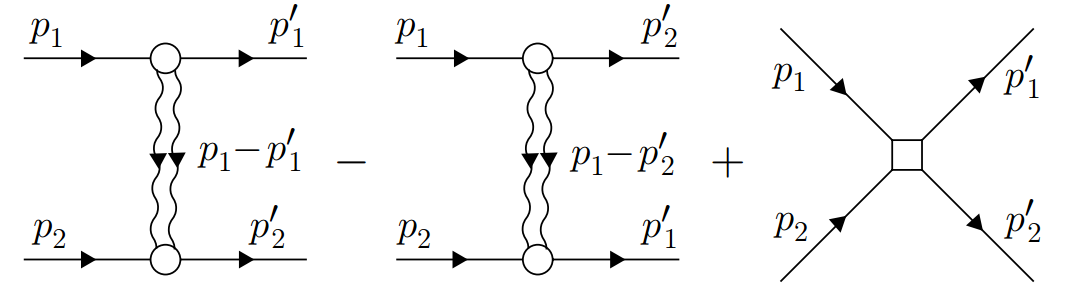
\includegraphics[scale=0.3]{QFT3/EES.png}
\caption{Diagrams for the exact electron-electron scattering amplitude. The vertices and photon propagator are exact; external lines stand for the usual $u$ and $\bar{u}$ spinor factors, times the unit residue of the pole at $p^2=-m^2$.}
\end{figure}
\\
In order to compute the contribution of these diagrams, we must evaluate $\overline{u}_{s'}(\bm{p}')\Gamma^{\mu}(p',p)u_s(\bm{p})$ with $p^2 = p'^2 = -m^2$, but with $q^2 = (p-p')^2$ arbitrary. Therefore we have 
\[\overline{u}_{s'}(\bm{p}')\Gamma^{\mu}(p',p)u_s(\bm{p}) = \overline{u}'_{s'}(\bm{p}')\left[F_1(q^2)\gamma^{\mu} - \frac{i}{m}F_2(q^2)\mathcal{S}^{\mu\nu}q_{\nu}\right]u_s(\bm{p}),\]
where we have defined the form factors
\begin{eqnarray}
F_1(q^2) &=& 1 - \frac{e^2}{16\pi^2} \int dF_3  \ln \left ( 1 + \frac{x_1x_2q^2/m^2}{(1-x_3)^2}\right ) \nonumber \\
&-& \frac{e^2}{16\pi^2} \int dF_3 \frac{1-4x_3+x_3^2}{(1-x_3)^2+x_3m_{\gamma}^2/m^2} + \frac{(x_3+x_1x_2)q^2/m^2-(1-4x_3+x_3^2)}{x_1x_2q^2/m^2+(1-x_3)^2+x_3m_{\gamma}^2/m^2} + O(e^4) ,\nonumber \\
F_2(q^2) &=& \frac{e^2}{8\pi^2} \int_0^1 dy \frac{1}{1 + y(1-y)q^2/m^2} + O(e^4) \nonumber
\end{eqnarray}
and
\[\mathcal{S}^{\mu\nu}= \frac{i}{4}[\gamma^{\mu},\gamma^{\nu}].\]
In on-shell renormalization scheme, we have $F_1(0) = 1$ and $F_2(0) = {\alpha}/{2\pi} + O(\alpha^2)$.

\subsection{Renormalization group}
\subsubsection{$\overline{\rm MS}$ renormalization scheme}
\[\Pi(k^2) = \frac{e^2}{2\pi^2} \int_0^1 dx \; x(1-x) \ln(\frac{x(1-x)k^2+m^2}{\mu^2}) + O(e^4).\]
\[Z_3 = 1 + \delta_3 = 1-\frac{e^2}{6\pi^2} \frac{1}{\epsilon} + O(e^4).\]
\[\Sigma(\slashed{p}) = -\frac{e^2}{8\pi^2} \int_0^1 dx  \ln(\frac{x(1-x)p^2 + xm^2 + (1-x)m_{\gamma}^2}{\mu^2}) \left((1-x)\slashed{p}+2m\right) + \frac{1}{2}\slashed{p} + m + O(e^4) .\]
\[Z_2 = 1 + \delta_2 =  1 - \frac{e^2}{8\pi^2}  \frac{1}{\epsilon} + O(e^4).\]
\[Z_m = 1 + \delta_m/m = 1 - \frac{e^2}{2\pi^2} \frac{1}{\epsilon} + O(e^4) .\]
\[\Gamma^{\mu}(p,p') = \gamma^{\mu} + \frac{e^2}{8\pi^2} \left[-\left(  1 + \frac{1}{2} \int dF_3 \ln (D/\mu^2)\right)\gamma^{\mu} + \frac{1}{4} \int dF_3 \frac{\tilde{N}^{\mu}}{D}\right] + O(e^4).\]
\[D = x_1(1-x_1)p^2 + x_2(1-x_2)p'^2 - 2x_1x_2p \cdot p' + (x_1+x_2)m^2 + x_3 m_{\gamma}^2.\]
\[Z_1 =1 + \delta_1 = 1 -  \frac{e^2}{8\pi^2}\frac{1}{\epsilon} + O(e^4).\]

\subsubsection{Renormalization group}
The Lagrangian of QED is
\[\mathcal{L} = -\frac{1}{4}F_{0\mu\nu}F_0^{\mu\nu} + \overline{\Psi}_0 (i\slashed{\partial}-m_0) \Psi_0 + e_0\overline{\Psi}_0\gamma^{\mu}\Psi_0 A_{0\mu}.\]
It can be written as
\[\mathcal{L} = -\frac{1}{4} Z_3 F_{\mu\nu}F^{\mu\nu} + \overline{\Psi} (iZ_2 \slashed{\partial}-Z_m m) \Psi + Z_1 e\overline{\Psi}\gamma^{\mu}\Psi A_{\mu}, .\]
Therefore,
\[\Psi_0 = Z_{2}^{1/2}\phi , \quad m_0 = Z_{2}^{-1} Z_{m}m , \quad A_0 = Z_3^{1/2}A , \quad e_0 = Z_{2}^{-1}Z_1 Z_{3}^{-1/2} e \tilde{\mu}^{\epsilon/2} = Z_{3}^{-1/2} e \tilde{\mu}^{\epsilon/2}.\]
After using dimensional regularization, the infinities coming from loop integrals take the form of inverse powers of $\epsilon$. 
In the  $\mathrm{\overline{MS}}$ renormalization scheme, we choose the $Z$s to cancel off these powers of $1/\epsilon$, and nothing more. Therefore the $Z$s can be written as
\begin{eqnarray}
Z_{1} = 1 + \sum_{n=1}^{\infty} \frac{a_n(\lambda)}{\epsilon^n} , \quad Z_{2} = 1 + \sum_{n=1}^{\infty} \frac{b_n(\lambda)}{\epsilon^n} ,\nonumber \\
Z_{3} = 1 + \sum_{n=1}^{\infty} \frac{c_n(\lambda)}{\epsilon^n} , \quad Z_{m} = 1 + \sum_{n=1}^{\infty} \frac{d_n(\lambda)}{\epsilon^n} .\nonumber 
\end{eqnarray}
In QED, $a_1 = -{e^2}/{8\pi^2} + O(e^4)$, $b_1 = -{e^2}/{8\pi^2} + O(e^4)$, $c_1 = -{e^2}/{6\pi^2} + O(e^4)$, $d_1 = -{e^2}/{2\pi^2} + O(e^4)$.
Remember that bare fields and parameters must be independent of $\mu$.
Define
\[E(e,\epsilon) \equiv \ln(Z_3^{-1/2}) = \sum_{n=1}^{\infty} \frac{E_n(e)}{\epsilon^n}.\]
We can get $E_1 = -{c_1}/{2} = {e^2}/{12\pi^2} + O(e^4)$.
As $\ln e_0 = E + \ln e + {\epsilon \ln \tilde{\mu}}/{2} $, due to the independence of $e_0$, we can derive
\[\left ( 1 + \frac{e E'_1}{\epsilon} + \cdots \right) \frac{d e}{d\ln \mu} + \frac{\epsilon}{2} e = 0.\]
In a renormalizable theory, we should have
\[\frac{d e}{d\ln\mu} = -\frac{\epsilon}{2} e + \beta(e).\]
Thus
\[\beta(e) = \frac{e^2}{2} E'_1(\lambda).\]
In QED, we have
\[\beta(e) = \frac{e^3}{12\pi^2} + O(e^5).\]
Define
\[M(e,\epsilon) \equiv \ln(Z_{m} Z_{2}^{-1}) = \sum_{n=1}^{\infty} \frac{M_n(\lambda)}{\epsilon^n}.\]
We can work out $M_1 = d_1 - b_1 = -{3e^2}/{8\pi^2} + O(e^4)$.
As $\ln m_0 = M + \ln m $, define the anomalous dimension of the mass
\[\gamma_m(e) \equiv \frac{1}{m} \frac{dm}{d \ln \mu}.\]
From the independence of $m_0$, we can derive
\[\gamma_m(e) = \frac{e}{2} M'_1.\]
In QED theory, we have
\[\gamma_m(e) = -\frac{3e^2}{8\pi^2} + O(e^4).\]
Expand $\ln Z_{2}$ as
\[\ln Z_{2} = \frac{b_1}{\epsilon} + \cdots\]
Define the anomalous dimension of the fermion field
\[\gamma_{2}(e) \equiv \frac{1}{2} \frac{d\ln Z_{2}}{d \ln \mu}.\]
We can derive
\[\gamma_{2}(e) = -\frac{1}{4}e b'_1.\]
In QED theory, we have
\[\gamma_2(e) = \frac{e^2}{16\pi^2} + O(e^4).\]
Expand $\ln Z_{3}$ as
\[\ln Z_{3} = \frac{c_1}{\epsilon} + \cdots\]
Define the anomalous dimension of the EM field
\[\gamma_{3}(e) \equiv \frac{1}{2} \frac{d\ln Z_{3}}{d \ln \mu}.\]
We can derive
\[\gamma_{3}(e) = -\frac{1}{4}e c'_1.\]
In QED theory, we have
\[\gamma_3(e) = \frac{e^2}{12\pi^2} + O(e^4).\]

\subsection{The magnetic moment of the electron}
Suppose there is a constant classical electromagnetic background field $A_{\mu}^{\mathrm{cl}}(\bm{x})$. Then we have a new term
\[e\gamma^{\mu}A_{\mu}^{\mathrm{cl}}(\bm{x}) \overline{\Psi}\Psi\]
in the Lagrangian. In Feynman diagram, this term joins two fermion lines. 
The value of the vertex is
\[ie\gamma^{\mu}\int d^4x e^{-i\bm{q}\cdot\bm{x}}e^{i(E'-E)t} A_{\mu}^{\mathrm{cl}}(\bm{x}) = ie\gamma^{\mu}\tilde{A}_{\mu}^{\mathrm{cl}}(\bm{q})(2\pi)\delta(E'-E).\]
where
\[\bm{q} \equiv \bm{p}' - \bm{p} , \quad \tilde{A}_{\mu}^{\mathrm{cl}}(\bm{q}) \equiv \int d^3x e^{-i\bm{q}\cdot\bm{x}} A_{\mu}^{\mathrm{cl}}(\bm{x}),\]
If an electron scatters in the background field and its momentum changes from $p$ to $p'$, then the scattering matrix is
\[\langle \bm{p}' | S | \bm{p} \rangle = ie\overline{u}_{s'}(\bm{p}')\Gamma^{\mu}(p',p)u_s(\bm{p})\tilde{A}_{\mu}^{\mathrm{cl}}(\bm{q})(2\pi)\delta(E'-E).\]
If there is only magnetic field, we have
\[A_{\mu}^{\mathrm{cl}}(x) = (0,\bm{A}_{i}^{\mathrm{cl}}) , \quad \bm{B} = \bm{\nabla} \times \bm{A}^{\mathrm{cl}}.\]
In momentum space, we have
\[\tilde{\bm{B}}^{\mathrm{cl}}(\bm{q}) = i\bm{q}\times\tilde{\bm{A}}^{\mathrm{cl}}(\bm{q}).\]
Recall that
\[u(\bm{p}) = D(\Lambda)u(\bm{0}),\]
where $\Lambda$ boost the the four momentum $(m,\bm{0})$ to $(E,\bm{p})$.
In the non-relativistic limit, we keep only the first order of momentum. The rapidity for the boost is $\bm{\beta} = {\bm{p}}/{m}$ and
\[D(\Lambda) = I + \frac{i}{2}\delta\omega_{\mu\nu}\mathcal{S}^{\mu\nu} = I + i \beta^i \mathcal{S}^{i0} = I - \frac{1}{2m} \begin{bmatrix} p^i \sigma^i  &0\\0& -p^i \sigma^i \end{bmatrix} .\]
Thus
\[u(\bm{p}) = \sqrt{m}  \begin{pmatrix}(1 - \bm{p}\cdot\bm{\sigma}/2m)\xi\\(1 + \bm{p}\cdot\bm{\sigma}/2m)\xi\end{pmatrix} ,\]
where $\xi$ is the state of electron spin. 
We can get
\[\bar{u}(\bm{p}') \gamma^i u(\bm{p}) = 2m \xi'^{\dagger} \left( \frac{\bm{p}'\cdot\bm{\sigma}}{2m}\sigma^i + \sigma^i\frac{\bm{p}\cdot\bm{\sigma}}{2m} \right) \xi = 2m \xi'^{\dagger} \left( \frac{p_i + p'_i}{2m} -\frac{i}{2m}\epsilon_{ijk}q_j\sigma_k \right) \xi.\]
The first term in the bracket is spin-independent. It is the contribution of the operator $[\bm{p}\cdot\bm{A} + \bm{A}\cdot\bm{p}]$ in the standard kinetic energy term of non-relativistic quantum mechanics. 
The second is the magnetic moment interaction we are seeking. Thus we retain only the latter term in the following discussion.
On the other hand, we have
\[\bar{u}(\bm{p}') \left( - \frac{i}{m}\mathcal{S}^{i\nu}q_{\nu} \right) u(\bm{p}) = 2m \xi'^{\dagger} \left( -\frac{i}{2m}\epsilon_{ijk}q_j\sigma_k \right) \xi.\]
Therefore,
\begin{eqnarray}
\langle \bm{p}' | S | \bm{p} \rangle &=& 2ime \xi'^{\dagger} \left( -\frac{i}{2m}\epsilon_{ijk}q_j\sigma_k[F_1(0) + F_2(0)] \right) \xi \tilde{A}_{i}^{\mathrm{cl}}(\bm{q})(2\pi)\delta(E-E') \nonumber \\
&=& i(2m)\xi'^{\dagger} \left( \frac{e}{m}[F_1(0) + F_2(0)] \frac{\sigma_k}{2}\right) \xi \tilde{B}_{k}^{\mathrm{cl}}(\bm{q})(2\pi)\delta(E-E'). \nonumber
\end{eqnarray}
Recall in quantum mechanics, the time dependent perturbation theory gives the transition matrix in first order as
\[\langle \bm{p}' | iT | \bm{p} \rangle = -i\int_0^t dt e^{i(E'-E)t} \langle \bm{p}' | V(\bm{x}) | \bm{p} \rangle \to -i\times 2\pi\delta(E'-E)V(\bm{q}),\]
where $V(\bm{x})$ is perturbed potential we applied to free particles. Note that in quantum field theory, we normalize the momentum eigenvector as
\[\langle \bm{p}' | \bm{p} \rangle = (2\pi)^3 2E \delta(\bm{p}-\bm{p}') \]
rather than
\[\langle \bm{p}' | \bm{p} \rangle = (2\pi)^3 \delta(\bm{p}-\bm{p}')  .\]
Thus there is a extra factor $2m$ in the equation we derived by field theory. By comparison, we conclude that
\[V(\bm{q}) = -\xi'^{\dagger} \left( \frac{e}{m}[F_1(0) + F_2(0)] \frac{\sigma_k}{2}\right) \xi \tilde{B}_{k}^{\mathrm{cl}}(\bm{q}).\]
Therefore, the magnetic moment of electron is
\[\bm{\mu} = \frac{e}{2m}[2F_1(0) + 2F_2(0)]\bm{S}.\]
The $g$-factor is
\[g = 2F_0 + 2F_2(0) = 2 + \frac{\alpha}{2\pi}.\]

\subsection{Lamb shift}
Let us consider the scattering of distinguishable fermions, for example electron and proton, in the non-relativistic limit. 

\begin{figure}[!h]
\centering
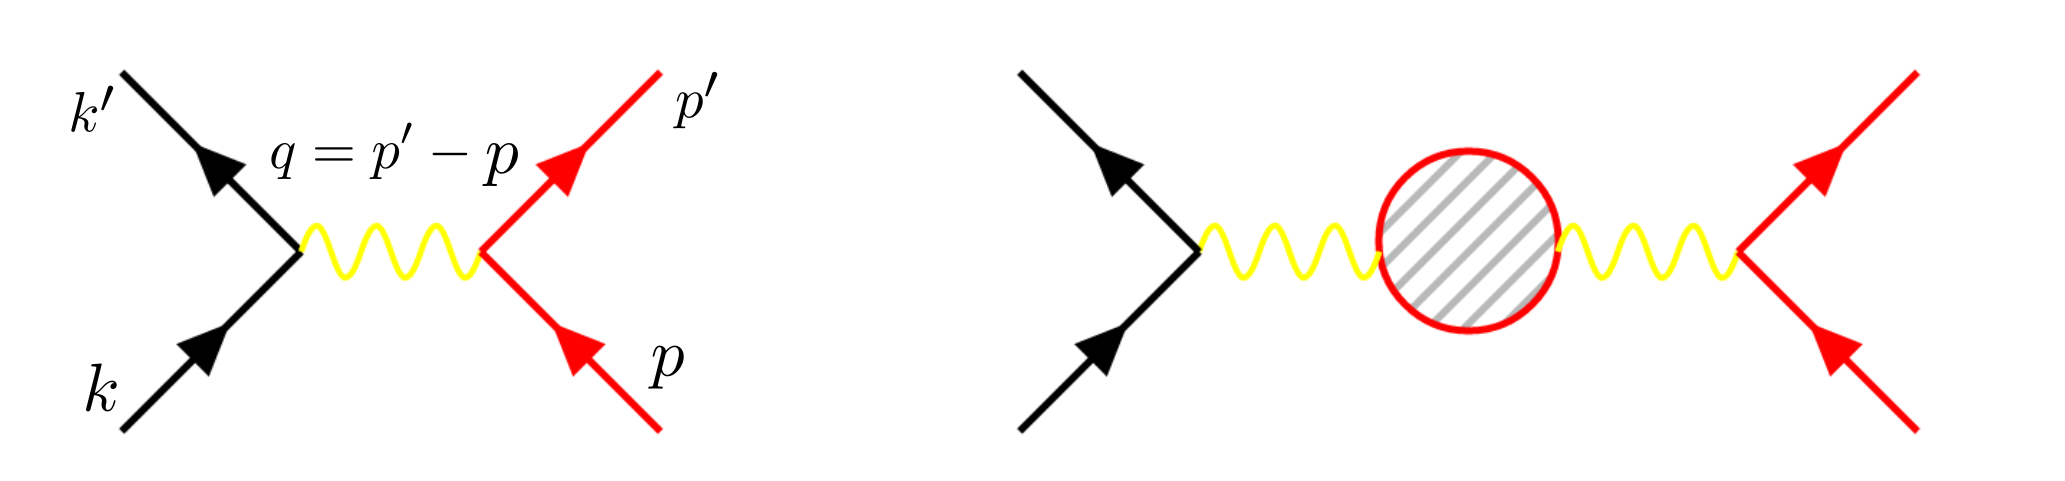
\includegraphics[height=3cm ,width=12.8cm]{QFT3/lamb.png}
\caption{Coulomb potential scattering} 
\end{figure}

\noindent
Up to tree level, we have
\[i\mathcal{M} = \bar{u}(k')(-ie\gamma^{\mu})u(k) \frac{-i\eta_{\mu\nu}}{q^2} \bar{u}(p')(ie\gamma^{\nu})u(p) = -i \frac{-e^2}{\bm{q}^2} 2m \delta_{ss'} 2m\delta_{rr'}.\]
By comparison to Born approximation in quantum mechanics, we have
\[\tilde{V}(\bm{q}) = \frac{-e^2}{\bm{q}^2}.\]
Transform the potential to position space, we can get
\[V(r) = \frac{-e^2}{4\pi r}.\]
It is the Coulomb potential of electron and proton.
\\ \\
Next let us examine how $\Pi(q^2)$ modifies the electromagnetic interaction. We have the modified potential
\[\tilde{V}(\bm{q}) = \frac{-e^2}{\bm{q}^2(1-\Pi(q^2))},\]
where
\[\Pi(q^2) = -\frac{2\alpha}{\pi} \int_0^1 dx x(1-x) \ln \left( \frac{m^2}{m^2 + x(1-x)q^2} \right).\]
In the limit of $|q^2|<m^2$, we have
\[\Pi(q^2) = \frac{\alpha}{15\pi}\frac{\bm{q}^2}{m^2} , \quad \tilde{V}(\bm{q}) = -\frac{4\pi\alpha}{\bm{q}^2} - \frac{4\alpha^2}{15m^2}.\]
Transform the potential to position space, we can get
\[V(r) = -\frac{\alpha}{r} - \frac{4\alpha^2}{15m^2} \delta(\bm{x}).\]
The correction term indicates that the electromagnetic force becomes much stronger at small distances. This effect can be measured in the hydrogen atom, where the energy levels are shifted by
\[\Delta E = - \frac{4\alpha^2}{15m^2} |\psi(0)|^2.\]
The wave function is non-zero at the origin only for s -wave states. For the 2S state, the shift is about $-1.123 \times 10^{-7}$ eV. Note that the energy level of fine structure is $E_{nj}$. This modified potential causes a split for degenerate levels of different $l$. This is a (small) part of the Lamb shift splitting.
A more precise correction is given by Uehling potential
\[\delta V(r) = -\frac{\alpha^2}{4\sqrt{\pi}r} \frac{e^{-2mr}}{(mr)^{3/2}}.\]
Thus the range of the correction term is roughly the electron Compton wavelength, $\frac{1}{m}$. 
Since hydrogen wave functions are nearly constant on this scale, the delta function was a good approximation.
We can interpret the correction as being due to screening. At $r > \frac{1}{m}$, virtual $e^+e^-$ pairs make the vacuum a dielectric medium in which the apparent charge is less than the true charge. 
At smaller distances we begin to penetrate the polarization cloud and see the bare charge. This phenomenon is known as vacuum polarization.
